% !TeX root = main.tex
\chapter{Paper-based semantic speech editing}\label{chp:paper}

% Need for paper
One of the findings from Chapter~\ref{chp:screen} was that some producers find their work environment noisy and
distracting, and do not like working with screens for extended periods. This leads many to print out transcripts of
speech recordings so that they can review and edit the recordings away from the screen and/or office.

% Advantage of paper
Working on paper offers a number of advantages over working on screens. Most of these are self-evident, but still
worth reviewing.  Paper is lightweight, portable and does not require any power, which allows users to work almost
anywhere.  It is not back-lit, so is easier on the eyes.  It can be navigated quickly, annotated freely whilst reading,
and individual pages can be laid out and easily compared.  Its physical low-tech nature also means that it is
intuitive, robust, durable and does not crash or lose data.  Reading from paper rather than a screen allows readers to
gain a deeper understanding, easily cross-reference other documents, and interleave reading and writing
\citep{OHara1997,Mangen2013,Singer2017}.

%Transcripts are often printed out because:
%- it is easier to read than on screen
%- allows portability,
%- allows annotation,
%- flexible spatial layout
%- quick navigation
%- cross-referencing,
%- reduces battery anxiety,
%- more trusted by non-tech-savvy users

%A similar process happens in the production of media content. The production workflow typically involves recording
%material, selecting which parts of that material to use, then editing the desired material down to the final output
%\citep{Baume2015}.  Many producers will `log' the material after it is recorded by writing transcripts of what was
%said.  This is either done themselves or using a third-party service. These transcripts help producers to recall what
%was said and when, identify themes, and make links between different parts of their content.

% Disadvantage of paper
Compared to digital media, working with a physical medium like paper introduces restrictions that make it more
difficult to copy, share, store and archive information. Printing a document breaks the link to its digital source, so
is normally a one-way process, where any information that is changed/added cannot is not fed back. Additionally,
freehand annotations are unstructured, and cannot easily be digitised and re-used. This forces users to manually
re-enter the information into a computer. In the case of radio production, this involves using a DAW to edit the audio
based on paper notes, which can be slow and tedious.

% Digital paper
There are a number of technological solutions that can be used to create a `digital bridge' between paper and
its digital source. These offer the possibility to combine the advantages of paper and digital workflows. Using this
approach, it is possible to link the words on a printed transcript of speech to the time they were spoken in the
original audio recording. Furthermore, by linking the paper annotations to audio edit commands, the paper could be used
to directly edit the audio content.

% Intro
In this chapter, we investigate paper-based workflows in the context of professional radio production. We describe how
we captured the requirements for a paper-based speech editor, and how we designed and built a working prototype. We
then describe a contextual study of radio production in which we directly compared screen-based and paper-based
workflows. 

\section{Background}\label{sec:paper-background}
Radio production using a paper interface requires a system that automatically translates annotations on a printed
transcript to audio edit commands. Such a system requires a method of linking paper to media.

`The Audio Notebook' \citep{Stifelman2001} was a system that used a physical pen and paper interface in combination
with a device that recorded audio synchronously with the page and vertical location of the written notes.  The device
could also replay the audio from a page and display which notes relate to the current playback position using an LED
scrollbar display at the side of the page. Users could also use the scrollbar to control the position of the audio
playback.  A longitudinal study of six participants over five months again found that users needed to take fewer notes,
and made more notes during replay. Two of the participants were reporters who used the system while recording
interviews. One reporter made minimal notes during the interview, but replayed the interview and made additional notes,
including star symbols to indicate important moments. They also extracted quotes of interest by typing them into a
computer. The other reporter was skeptical of the system, so made detailed notes so not to rely on the audio. However,
they were later able to use the system to recall bits of the interview, which was many times faster than their existing
technique of fully transcribing the audio recording.

We have identified three main approaches for achieving this, using barcodes, digital ink and digital pens.
In this section, we will review previous systems and studies that have used these techniques to link media with written
documents.

%\subsection{Screen-based}
%Transcript-based interfaces have already successfully been applied to both audio and video editing. SCANMail
%\citep{Whittaker2002} demonstrated the advantages of navigating voicemail recordings using a transcript, but did not
%include editing capabilities.  The LIDS Editor \citep{Apperley2002}, and later TRAED \citep{Masoodian2006}, used
%automatically-generated transcripts to allow users to navigate and edit lecture recordings by removing and rearranging
%sentences and words. Even though automatically-generated transcripts are imperfect, Whittaker and Amento found they are
%sufficiently accurate to allow navigation and editing \citep{Whittaker2004}.  More recently, Rubin \citep{Rubin2013}
%created a system for using editable crowd-sourced transcripts to create audio stories.  Similar techniques have been
%applied to video editing. SILVER \citep{Casares2002} was a video editor that had an editable transcript window,
%generated from subtitles, and Berthouzoz et al.  \citep{Berthouzoz2012} developed a system that used crowd-sourced
%transcripts and image processing to allow text-based editing of multi-camera video interviews.

\subsection{Barcodes}
Paper transcripts have been explored as a method of navigating video recordings by using a device to detect the
position in the text and play the video from that position. \citet{Hull2003} describes a system called `Video Paper',
which embedded video keyframes with barcodes down the side of the page. It used a PDA to scan the barcodes that linked
to a position in a video, which was downloaded and played on the device. \citet{Klemmer2003} applied Video Paper to
oral history in a project called `Books with Voices'. An evaluation of 13 users found that it had substantial benefits
with minimal overhead.  \citet{Erol2007} went a step further by embedding the video in the barcode data, removing the
need to download the video from a separate source. \citet{Erol2008} removed the need for barcodes by creating a system
called `HotPaper', which used a camera to measure the whitespace between words and matched that to unique patterns in
the text.

Barcode-based systems provide a link between text and media, however they do not provide a convenient method of
capturing annotations. It would be possible to use a PDA-style device to capture annotations and link them to a
particular barcode. However, this requires that the annotation are entered into a handheld device, rather that just
written on the paper. Additionally, the size of the barcodes means that the precision of the timestamps would be at a
sentance-level rather than word-level.

\subsection{Digital ink}
`Digital ink' refers to technology that digitally captures and responds to the moments of a pen, such as a stylus on a
tablet PC.

\subsubsection{Synchronised note-taking}
`Marquee' \citep{Weher1994} was a digital ink system for supporting the task of logging during a live video recording.
Users could make synchronised handwritten notes by drawing a horizontal line to mark a timestamp, then writing their
notes below.  Additionally, they could create a list of keywords, and add them to their notes by pressing them at the
right moment.  Marquee was evaluated for note-taking during meetings with three participants. The study found that
users did not partake in discussions while logging, which may prevent such a system being used during an interview.
The freehand nature of the notes meant that it could easily handle the different styles of each user.  Users reported
that they didn't feel they had to make as many notes as they normally would, because they could later refer back to the
video recording. The authors also noted that videos can be further annotated during replay, allowing for an iterative
logging process.

`Dynomite' \citep{Wilcox1997} was a virtual notebook that recorded audio synchronously with digital ink handwritten
notes. The user's notes could be assigned to different `properties', either before or after they were written, to
indicate an action point, for example, or a user-specified keyword.  Users could also highlight a portion of the audio
by pressing a `mark' button or making a specific gesture.  This would highlight the audio for a specified time period,
unless the `extend' or `end mark' buttons were pressed.  Any notes made during this period were displayed in bold and
the highlighted segments were displayed using colours on a horizontal timeline. An evaluation of nine users found that
users took fewer notes when using the audio highlighting, and that they wanted to go back and use the audio to improve
the notes afterwards. Both of these findings mirror those from \citet{Weher1994}.

\subsubsection{Video editing}
Several systems have experimented with using pens with interactive sliders to provide advanced control for
navigating video content, such as `LEAN' \citep{Ramos2003}, `Zlider' \citep{Ramos2005} and MobileZoomSlider/ScrollWheel
\citep{Huerst2008}. However, these systems are limited to the navigation of content, without changing or labelling it.
Our interest is primarily in the annotation and editing of media, which the following systems have explored using
digital ink interfaces.

\citet{Diakopoulos2006} created a digital ink interface for creating and annotating segments of a pre-recorded video,
called `VideoTater'. Segments could be created by drawing a vertical line on a video timeline, and merged by drawing a
horizontal line between them. Each segment could be tagged by selecting it and hand-writing text. The back of
the pen could be used to erase tags. Pen pressure was used to distinguish between selection and tagging, with low
pressure for selecting and high for tagging. Informal feedback from three users found that the gestures were
successful, and that the pressure mapping worked well.

\citet{Cattelan2008} added functionality for marking edit commands using digital ink in their system `WaCTool'. The
system included a variety of features for annotation, editing and real-time collaboration. Users could use a pen to
write annotations by tapping the video to freeze it, then drawing on the video frame.  Users could apply a `skip'
command to a segment of the video by using the pen to tap the bottom left of the video at the start of an unwanted
segment, and tapping the bottom right at the end. The `skip' command is analogous to editing out part of the video.
Similar commands for looping and slow motion were also available by tapping different regions.

`Video as Ink' \citep{Cabral2016} took an alternative approach by allowing users to `paint' video frames and segments
onto a 2D canvas using a pen and tablet interface. The canvas works as a timeline, but extends vertically in both
directions so that the video can be painted onto multiple rows. The system includes gestures for adding, moving,
erasing and selecting content. An evaluation of 12 participants found that the canvas allowed users to creatively
explore different possibilities. However, the interface relies on the visual organisation of images, which does not
necessarily translate well to audio and text.

\subsubsection{Proof-reading}

\citet{Yoon2014} created a collaborative digital ink document annotation system called `RichReview', which offered
users three modalities in which to annotate documents - freeform inking, voice recording and deictic gestures. The
voice recordings were displayed using a waveform, overlaid with an automatically generated transcript of the speech.
Users could trim or tidy the voice recordings by drawing a line through words or pauses to remove them.  The system was
evaluated using a qualitative study of 12 students which found that the editing features were considered easy to use
and efficient for removing `umm's and long pauses.  However, many participants reported that the transcripts were not
accurate enough to use without having to listen to the audio.

\subsection{Digital pens}
A digital pen looks and functions as a normal pen, but includes an on-board infrared camera that tracks the position of
the pen while it writes on paper. Digital pens must be used in combination with paper that has a unique non-repeating
dot pattern printed onto it using a standard colour laser printer.  By reading this pattern, the pen can calculate
exactly where it is when touching the page. This information is captured up to 100 times a second and recorded
digitally onto the pen. Depending on which pen and which software you're using, this information can either be streamed
live via Bluetooth, or downloaded as a batch onto a computer. This technology has been patented by Anoto Group
\citep{Fahraeus2003}, who exclusively manufacture and licence digital pen products. As such, this technology is often
referred to as the `Anoto dot pattern'.

% Pens
%Livescribe Pulse
%Live Pen 1 (DP-201)
%Live Pen 2

\subsubsection{Proof-reading}

\citet{Guimbretiere2003} introduced a concept called `PADD', which was a system of editing documents that uses the
Anoto pattern to allow users to move from digital documents to paper and back again. \citet{Conroy2004} created
`ProofRite', which was the first full implementation of a PADD system. It captured annotations made to a printed text
document, and overlaid the annotations onto the text in a word processor. The annotations were anchored to the text,
such that they `reflow' when the text is moved. Through informal feedback, users suggested that their annotations
should translate into actions such as delete.

\citet{Weibel2008} created `PaperProof', which interpreted the edit annotations and automatically applied them to the
document. Gestures for delete, insert, replace, move and annotate were translated into modifications in a word
processor, and intelligent character recognition was used to digitise any hand-written text. Processing the annotations
allows for a two-way interaction between the digital and paper representations. There were no user studies of the
PaperProof system.

\subsubsection{Synchronised note-taking}

ChronoVis \citep{Fouse2011} used the Anoto dot pattern to record paper notes during playback of a video. The on-screen
playback interface allowed users to click on the digital display of the handwritten notes to navigate to that position
in the video, or browse a list of timestamped notes. Alternatively, they could reprint their notes and use a
wirelessly-connected digital pen to tap on the notes, which controlled the playback position.
ChronoVis can also coordinate multiple data sources, such as GPS logs.

\citet{Weibel2012} conducted a longitudinal study of ChronoViz for use in observational research. They studied how
three research groups used the technology over a period of 18 months by observing their use of ChronoVis, and
conducting regular focus group and brainstorming discussions.  The study found that the introduction of the system
changed the note-taking practices of the participants.  Notes became a mixture of linear notes and symbolic
representations.  Asterisks, stars and simple shapes were used as bookmarks for later referral.  Strokes in certain
areas of the paper were used to capture structured data. Single strokes were used for binary data (like a checkbox),
multiple strokes were used for counting events, and handwriting was used for categorical data.  One research group
stopped manually writing the time as they normally would, because this information was captured automatically. The
flexibility of freehand notes also enabled use of arrows in various contexts such as to indicate direction and actions.

Paper-digital notes introduce time as an additional structuring factor, and the authors discuss the tension between the
use of time and space. They point out that `deciding when time, space or both are important in a paper-digital form is
complex'.  One benefit of a paper-digital interface is that when the digital pen fails, the paper still contains
important information, however this is not true for time information.

Based on feedback from this study, ChronoVis was enhanced with features to control video playback, automatically
recognise specific symbols and add notes on top of existing notes.

% Sensitivity of zones - a line which crosses from one zone to another can be a problem.
% Problems when line or symbols crosses over zone

%\subsection{Synchronised note-taking}
%A number of previous systems have explored how media can be annotated as it is recorded or replayed. These have often
%been developed for note-taking during meetings or lectures, but could also be applied to radio production. Although we
%did not find that it was commmon to write notes during interviews, we found that producers often listen back to their
%recordings, so these systems could be using during that replay process.

%\subsection{Correction}
%In chapter~\ref{chp:screen}, we identified that some producers were interested in correcting the transcript for sharing
%with others, or for later publication.

%TODO There are clearly defined symbols for use in proof correction (e.g. \citet{ISO5776}).

%TODO Interfaces to correct errors in transcripts have also been considered, such as that from \citet{Suhm2001}.

\subsection{Summary}

% MECHANISMS
% - digital ink vs digital pen vs barcode
In this section, we have seen how barcodes, digital ink and digital pens have been used to link written documents to
timed media.

Barcodes provide a simple mechanism for linking physical printed paper to digital media. This provides the
benefits that come with reading from and annotating paper, but with a link to the source media. The barcodes are easy
to generate, don't need a licence and are robust to photocopying.  We need a device to read the barcodes, but we
could do this using the camera on a mobile phone.  The systems to date have only provided a one-way link from paper to
media.  It would be possible to implement a feedback mechanism, but the data would have to be entered into the scanning
device rather than the paper. This means that the freehand annotation are not supported, not would they be accessible
without using the device. Barcodes also take up a lot of space, so it is only practical to have them at the end
of a line, rather than for each word. This limits the precision with which they can be used.

Digital ink interfaces are vastly more feature-rich as they use a device with a screen that is capable of advanced
two-way interaction. The device can integrate with media playback to allow users listen to the audio. Freehand
annotations can be used to annotate documents, and these can easily be undone or erased. Pressure mapping can also be
used to interact in several different modes.  However, digital ink interfaces use screens rather than physical paper,
so do not benefit from improved comprehension and cross-referencing. The screen in digital ink devices mean that they
are often bulky and have a short battery life. Additionally, because the device must be used to access the information,
this is lost in the event of device failure.

Digital pen interfaces combine most of the benefits of both barcode and digital ink interfaces. They use physical
paper, which is better for reading, but also allow a two-way interaction with freehand annotation. The pen-based
interface is very natural and familiar, and because the annotations are made on the paper itself, information is both
accessible and backed-up in the event of device failure. However, there are some limitations to digital pen systems.
A colour laser printer must be used with proprietary software to print the required dot pattern, and the printouts
cannot be photocopied. There is no easy way to undo or erase annotations, although this is an inherint problem with
pens in general.

Electronic paper is a technology that attempts to emulate the benefits of reading from paper. Although it has been
commercially successful through its use in e-readers, studies have found that e-paper has a higher reading time, worse
comprehension and higher eye fatigue than reading from normal paper \citep{Jeong2012, Daniel2013}.
Additionally, we could not find any systems that provided the digital ink interaction that would be needed to mark-up a
transcript.

%TODO GAP IN LITERATURE
% - previous paper or pen-based systems have concentrated on navigation and annotation
% - some simple editing functionality was present in digital ink systems, but these didn't use transcripts
% - PaperProof allowed editing of text, but this didn't link to media
% - haven't considered audio, only audio-visual; not always translatable (e.g. video as ink)

We have seen that digital pen technology has successfully been applied to text editing \citep{Weibel2008} and media
annotation \citep{Fouse2011}. We could not find any previous literature which has combined these approaches by linking
text to the transcript of recorded speech.

Video editing functionality was present in \textit{VideoTater} \citep{Diakopoulos2006}, \textit{WaCTools}
\citep{Cattelan2008} and \textit{Video as Ink} \citep{Cabral2016}. However, all of these systems relied on the
manipulation of video thumbnails, which cannot be translated to audio editing. None of them considered text or
transcript-based editing.

% Time dimension - time vs spatial representation

% Multiple iterations

\section{System requirements}\label{sec:paper-requirements}

% Decided to use digital pens
In the background section, we found that digital pens have successfully been applied to text editing and media
annotation. We aimed to combine these into a paper-based audio editing system for radio production. We hoped this
would combine the portability, familiarity and readability of paper with the efficiency of text-based audio editing. 

% Collaborated with Anoto
Digital pen technology is based on a set of techniques that are protected by a number of patents \citep{Fahraeus2003}.
These are owned by Anoto Group, who exclusively license this technology and manufacture a number of products. Creating
custom solutions can be expensive, so we collaborated with Anoto to develop our audio editing system. The system was
based on their Live Forms platform, which is designed for processing documents to capture digital information from
handwritten annotations.

In order to build our system, we needed to design the layout of the document and define a set of gestures for
editing the content.  As there were no previous systems on which to base our design, this process raised a number of
questions about what information we should include in the layout, and which gestures we should use for interaction.
Specifically we were interested in answering the following questions:

{\singlespacing
  \begin{itemize}
    \item What gestures are currently used by radio producers to annotate transcripts?
    \item Do producers prefer to select content they want to keep, remove content they don't want, or a mixture of the
      two?
    \item Which additional features (e.g. timestamps, speaker labelling, confidence shading) should be included in the
      layout?
  \end{itemize}
}

To try and answer these questions, we created a paper prototype of our paper interface. The prototype used a normal pen
rather than a digital pen, so did not process the gestures, but the paper prototype gave an almost identical
expeirience. This allowed us to test an initial design of our interface with users before building the functional
system.  In this section, we describe the design of our paper prototype, explain how we evaluated it and outline our
findings.

\subsection{Paper prototype design}

% Transcript, from speech-to-text system
We based the design of our prototype around a printed transcript, which we enhanced with additional information and
arranged to simplify the capture of structured annotations. An example of the design is shown in
Figure~\ref{fig:paper-prototype-design}.

\begin{figure}[h]
  \centering
  \includegraphics[width=\columnwidth]{figs/paper-prototype-design}
  \caption{Design of the paper prototype}
  \label{fig:paper-prototype-design}
\end{figure}

The transcript was generated using an automated speech-to-text system, which contained ocassional errors. We chose to
use this rather than a perfect transcript as we wanted to use automated transcription for the final system, and
removing the errors may affect user behaviour.

% Limitations of Anoto system, used normal pen for prototype
The Anoto Live Forms platform, which we used to create our system, works by dividing the page into rectangular active
zones.  When a digital pen draws inside one of these zones, that data can then be captured digitally and processed.
Traditionally this is used to detect when someone has ticked a box on a form, or to extract an image of a signature
drawn inside of a box.  To capture edit annotations that linked to the text of the transcript, we designed our layout
to use rectangular active zones that aligned with the location of each word.

% Edit commands: selector beneath word (double-spaced) and at end of line, removal by crossing word
From what we had witnessed from previous experiments, the most common annotations producers used were underline,
strikethrough and drawing a line down the side of the page.  To capture strikethrough, we drew an invisible active zone
on top of each word, so that when a line is drawn through the word, the zone is triggered. For underline, we draw a
shaded active zone directly below each word, so that drawing a line underneath a word triggers the zone. The transcript
was printed double-spaced to leave enough room for these boxes. Finally, we draw a shaded active zone at the end of
each line. Drawing a line through this zone would select the whole line.

% Additional features: paragraphs and speaker ID with gender, timestamp at start of line, confidence shading
The speech-to-text system we used provided additional information with the transcript.  Each word came with a timestamp
and a confidence rating. We wrote the timestamp at the beginning of each line in \textit{MM:SS} format, and used
confidence shading to grey-out lower confidence words.  The speech-to-text system also used speaker diarization
techniques to segment the transcript by speaker. This provided a speaker label and estimated gender for each segment.
We used paragraphs to segment the transcript, and wrote the speaker label at the start of each paragraph. We used blue
colouring for male speakers, and red for female speakers.

\subsection{Evaluation method}

%TODO Explain interview protocol and analysis

%TODO Why are participants asked to adopt three different strategies?

%TODO Explain design decisions, e.g. double-spacing, confidence shading

To evaluate our paper prototype, we ran a short experiment in which radio producers used our inactive prototype to
annotate real transcripts as if they were editing them.  We asked them to edit the transcripts in different ways, and
interviewed them afterward to compare the various approached. Producers are very busy, so to gain enough participants
in the time we had available, we designed the experiment so it could be completed within an hour.

We recruited five producers by using the contacts that we made from previous experiments. Two of the participants
worked in current affairs, two in science and one in documentaries.  The participants had between 7 and 13 years
experience working as a radio producer.

For the transcript, we asked each participant to provide us with a recent interview they had made, which we ran through
our speech-to-text system. We used this automated transcript for each participant's experiment so that they were
working with authentic speech, and a transcript that would be the same as that from a working system.

To help explore our questions about annotation and editing gestures, we directed participants to employ three different
strategies when using the prototype. This forced them to experience different ways of interacting with the prototype,
which they could later reflect on and compare. We instructed them to follow these directions for the first three
pages of their transcript: 

\begin{itemize}
  \item \textit{Page 1}: Undirected\\Edit the speech by annotating the transcript as you would normally.
  \item \textit{Page 2}: Underline only\\Edit the speech only by underlining words that you want to keep.
  \item \textit{Page 3}: Strikethrough only\\Edit the speech only by putting a line through words you don't want to keep.
\end{itemize}

The `undirected' strategy allowed us to see what gestures producers currently use, or want to use, without being
influenced by the design of the prototype or constrained by its limitations. We included the underline and
strikethrough strategies as we believed these to be the two most commons approaches, and we wanted the participants to
compare them directly.

We were also interested in learning about additional features and their value. To get feedback on the value of speaker
diarization, we produced two versions of each participant's transcript -- one with speaker diarization and one without.
The speaker information was used to segment the transcript into paragraphs, and the start of each paragraph was
labelled with the speaker identifier in square brackets (e.g.  \texttt{{[}S1{]}}).  For \textit{Page 4}, each
participant was presented with a transcript that included speaker diarization, and asked to edit the speech by
annotating the transcript any way they wished.

Timestamps, line selection and confidence shading were included with all of the prototypes. For these features, we
chose not to produce versions with/without as participants should be able to judge their value without having to see
them removed. Producing different versions for each would also unduly lengthen the experiment.

At the end of the test, we conducted a semi-structured interview with each participant. The following questions were
asked, but we also let the participants talk about whatever else they wanted to.

{\singlespacing
  \begin{itemize}
    \item How do you normally use a pen to edit the transcript?
    \item Do you prefer to select parts you want to keep, or remove parts you don't want to keep?
    \item Which features of the prototype did you find useful?
    \item Were there any features missing that you would want added?
  \end{itemize}
}

The experimenter wrote down the participants responses from the interview. These were then categorised into natural
gestures, edit gestures and additional features. We counted the frequency of each response within the categories to
see how popular the different approaches and features were. The participant's annotated transcripts were also
collected.

\subsection{Results}
The reaction to the system was overwhelmingly positive. All of the participants could immediately see the value of such
a system and most remarked that it would save them significant amounts of time and \textit{``revolutionise''} their
production workflow.

\subsubsection{Natural gestures}

The participants started the experiment by editing the transcript using any gestures they wanted.
Table~\ref{tab:natural-gestures} lists the gestures that were used, and by which participants.

\begin{table}[ht]
  \centering
  \begin{tabular}{|l|c|c|c|c|c|c|}
    \hline
    & P1        & P2        & P3        & P4        & P5        & Count \\
    \hline
    Underline               & $\bullet$ & $\bullet$ & $\bullet$ & $\bullet$ &           & 4 \\
    \hline
    Strikethrough           & $\bullet$ & $\bullet$ &           & $\bullet$ & $\bullet$ & 4 \\
    \hline
    Line down side          & $\bullet$ & $\bullet$ & $\bullet$ &           & $\bullet$ & 4 \\
    \hline
    Comments                & $\bullet$ & $\bullet$ &           &           & $\bullet$ & 3 \\
    \hline
    Correction              & $\bullet$ &           &           &           & $\bullet$ & 2 \\
    \hline
    In/out marks            & $\bullet$ &           &           & $\bullet$ &           & 2 \\
    \hline
    Scribble-out mistake    &           & $\bullet$ & $\bullet$ &           &           & 2 \\
    \hline
    Lasso                   &           &           &           &           & $\bullet$ & 1 \\
    \hline
    Line through paragraph  &           &           &           &           & $\bullet$ & 1 \\
    \hline
  \end{tabular}
  \caption{Natural gestures used by each participant to edit their transcripts}
  \label{tab:natural-gestures}
\end{table}

\begin{figure}[h]
  \centering
  \includegraphics[width=\columnwidth]{figs/mockup-cropped}
  \caption{Paper prototype with natural annotations, including
    underlining, line down the side with notes, word corrections, and a
  vertical line to indicate the end of an edit.}
  \label{fig:natural}
\end{figure}

Four different gestures were used to select content -- underline, line down side, in/out marks and lasso.  Underline
was used by all participants but one, who was mainly interested in deleted unwanted content.  Drawing a line down the
side was used by three participants, as it is quicker and more efficient than underlining for selecting large chunks of
material.  Some participants combined both by using underline to be more precise about the start and end of their
selection.  One of the participants made a mistake when underlining, so scribbled out the underline to undo it.

`In/out marks' refers to drawing short vertical or diagonal lines before and after the words of a selection. These
indicate the in- and out-points for edits. One participant drew an analogy between these marks and the splicing of
magnetic tape, which was how radio programmes were edited before the digital age. `Lasso' refers to selecting a number
of words by drawing a line around them.

Two gestures were used to delete content -- strikethrough and drawing a line through a paragraph. These parallel the
underline and line down side gestures that are used for selection, but instead involve drawing a line through the words
themselves.
%TODO Expand

Finally, two participants corrected mistakes in the transcript by writing the correction over/above the
word, or to the side of the page.
%TODO Expand

Each participant used a different mixture of annotation techniques.
%TODO Expand

\subsubsection{Edit gestures}\label{sec:paper-proto-edit-gestures}
We asked each participant whether they preferred selecting or deleting words for editing the transcript.  P1, P3 and P4
reported that they preferred selecting, P1 commented that it \textit{``felt more natural''} to them and P4 said
deleting felt \textit{``counter-intuitive''}.

P2 and P5 reported that they preferred deleting words. P2 commented that \textit{``the challenge is to nibble away''}
and it was \textit{``the way my brain works''}. P5 said they prefer to \textit{``get stuff out of the way''}.

All of the participants were certain about which they preferred, but there was no overall consensus. Additionally, we
can see in Table~\ref{tab:natural-gestures} that all participants used a mixture of select and delete gestures during
the undirected annotation.

\subsubsection{Additional features}

% speaker diarization
Four of the five participants said that they found the paragraphs and speaker information useful. Typically, interviews
are recorded with a presenter and contributor, and the participants said they found it valuable to know when the
presenter is asking a question. Three of the participants said that they were able to find the questions much more
easily with this feature enabled. However, P2 said they found the speaker diarization to be \textit{``distracting''},
particularly when it was inaccurate.

% timestamps/confidence shading
All participants found the timestamps and confidence shading features useful, but P2 said that the timestamps are
\textit{``not needed on every line''} and P5 suggested that one timestamp per page would be sufficient. All of the
participants liked being able to select whole lines at a time. P5, who prefers to remove words, asked whether a similar
function could be available to delete content.

\subsubsection{Missing features}

During our testing, some participants suggested adding features that were not included, or used the prototype in a
way it was not designed.
% highlighting
P3, P4 and P5 remarked that they often highlight important bits of transcripts, usually with asterisks or stars.
P1 and P3 also suggested that the underline gesture could be extended so that underlining words twice marks them as
being more important.

% labelling, margins
Three participants made notes on the side of the page to label their content or to make a note for themselves. Due to
the limited space, the notes were often scrawled sideways in small writing. If the prototype was active, writing notes
on the transcript itself would likely have triggered the active zones located on and below each word. This would cause
the user to inadvertantly create edits to the audio. P3 suggested that it may be worth adding a margin. Providing an
inactive margin would give users a `safe space' to make freehand notes without editing the audio.

% correction
Two participants corrected words in the transcript by writing over or above the incorrect word. As the transcript was
double-spaced, there was just enough room between lines to write the correct word in small writing.
% listening/playback
P3, P4 and P5 expressed a desire to listen to the audio while reading/editing it, which echoes the importance of
listening noted in Chapter~\ref{chp:screen}.

%- Useful to know where presenter is asking question

%Diarization
%- Neal found it easier
%- Shows where the questions are
%- Phil found it distracting
%- Wes found it absolutely useful
%- Marnie 'made it much easier', liked having paragraphs (usually one point per
%paragraph)


%Timestamps
%needed every couple of minutes

%Use L/R channels for presenter/contributor
%- Phil and Wes
%- Sometimes multiple on R channel (about one in eight interviews)

%Prefer landscape to portrait (landscape is `irritating' and doesn't match
%what's on screen)

%Whole line
%- Would like to delete line at a time

%Note-taking
%- One doesn't take many notes

%Correction
%- One corrects then selects edits
%- Wes would like option

%Highlighting
%- Asterix/star to mark important bits (Phil, Neal)
%- Underline twice (Neal, Marnie liked idea)
%- Wes sometimes double-stars

%Delete vs select (2 vs 3)
%- Phil likes to `get stuff out of the way'
%- Words that aren't marked should be kept by default
%- Underline should undo delete
%- Neal prefers selecting over deleting
%- Delete should undo select, if underlined too far
%- Wes prefers selecting - deleting is `counter-intuitive'
%- Would like delete to override select, but would like options for opposite
%- Marnie found it trickier to delete than select, selection is more natural
%- worried about deleting something good
%- Alex feels delete is more natural, 'way may brain works, 'challenge is to
%nibble away', thinks delete should be active, select should override delete

%Margin
%- Phil wouldn't need a margin
%- Neal would like one

%Export
%- gaps should be put between edits (real-time?)

%Transcript
%- Phil and Neal no problems
%- Wes had problems (strong Scottish accent) made it unusable

%Observation
%- Neal
%- underlined as he read (unprompted), scribbled out when mistake made
%- found it more difficult to only delete
%- Wes
%- vertical lines for in/out points

%Other
%- Neal would like to press and hear word (on laptop?)
%- Wes: Don't know what sounds good
%- Wes works in a team of 3/4. They use Box to collaborate
%P4 reported that they usually work in teams of 3 or 4 people. They use Google Docs to collaborate on a central
%programme script, so they can all edit the document simultaneously.

\subsection{Discussion}

In this section, we set out to answer three questions about the gestures producers use to edit printed transcripts, and
which features we should include in our paper-based audio editing interface. We did this by evaluating a paper
prototype of our interface on five radio producers using real content.

%\item What gestures are currently used by radio producers to annotate transcripts?
%\item Do producers prefer to select content they want to keep, remove content they don't want, or a mixture of the
%two?
%\item Which additional features (e.g. timestamps, speaker labelling, confidence shading) should be included in the
%layout?

We observed that the participants used a variety of gestures to select and delete content, with underline,
strikethrough and a line down the side being the most common.  This confirms our assumptions about these being the most
popular annotations, which drove the design of our prototype.  The other gestures included in/out marks and lasso for
selection, and drawing a line through a paragraph for deletion.  In \citet{Weibel2008}, strikethrough was also used for
delete, but something similar to in/out marks was used for annotating a specific region.

There were mixed but strong opinions on whether it was better to select good content or remove bad content.  Most
participants used a mixture of both approaches when undirected. Given the lack of consensus, it would be best to give
producers the option to do both, but this raises the issue of what should happen when a word is both selected and
deleted.  If one overrides the other, then it could function as an undo mechanism. The more conservative approach would
be for selection to override deletion, so that speech can always be recovered. However the system does not delete any
audio, so this is not a risk.

Selection and deletion could be used together at different scales, where one is used to select/delete large chunks,
then the other is used to refine the choise by selecting/deleting smaller words or chunks within the larger ones. In
our results, we saw that selecting large chunks is more popular than deleting large chunks. Also, there is likely to be
more interest in removing individual words, such as for `de-umming', than there is for selecting individual words. For
this style of use, it may be better for delete to override select.

When underline is used to select content, it implies that everything else should be discarded except for the underlined
parts. Alternatively, underline could be used to highlight parts of interest. In a later stage, the user could then
choose to either keep everything except the deleted words, or to keep only the highlighted words minus the deleted
words. This would give greater flexibility to different modes of use, like we saw in
Section~\ref{sec:paper-proto-edit-gestures}.

Most participants valued the additional features we tested -- speaker diarization, timestamps and confidence shading,
but reported that timestamps on every line are unnecessarily frequent. During our testing, we also identified missing
functionality for labelling, correction, highlighting and playback.

% Missing features
Handwritten text was also used to make
corrections to the transcript, and to label parts of the transcript.

% labelling
Three participants made notes on the side of the page to label their content or to make a note for themselves. Two of
the participants remarked that there was no free space in which to make notes, and suggested that it may be worth
adding a margin. Writing notes on the transcript itself would trigger the active zones that are on and below each word.
Providing an inactive margin would allow users to make freehand notes without inadvertantly making edits to the speech.

% correction
Two participants corrected words in the transcript by writing over or above the incorrect word. 
Potentially users could write the replacement word in an active zone, but...

% highlighting
Most participants remarked that they normally mark important bits of the transcript, often with asterisks or
stars. Underlining twice could also introduce a two-tier selection system.
Possibly the side boxes could be used to rate or star a selection.

% playback
Some participants expressed a desire to listen to the media from the paper interface, and this functionality has been
shown to be useful in previous work. %TODO Reference
An external device, such as a phone, computer or portable media player could be used to replay the audio while using
the paper interface.

Users could start playback by pressing a word with the digital pen. This could be
achieved either by wirelessly linking the digital pen to a computer that plays the content, or by storing the audio on
the pen itself similarly to the LiveScribe Sound
Stickers\footnote{\url{http://store.livescribe.com/sound-stickers-1-1.html}}.

% natural annotation:
% underline, strike and line down side most used, reinforced design decision
% comments and correction were popular, no space to write them
% in/out marks, lasso also used for selection, line through paragraph used for deletion, but to lesser extent

% edit gestures:
% no consensus on best approach, both used when naturally annotating, so both should be available
% what to do when using both? underline override strike or vice-versa?

% additional features:
% speaker diarization - yes
% timestamps - yes, but less frequently
% confidence shading - yes


%Our system performs the same function as these systems, but uses a paper
%interface rather than a screen-based one.
%Our system
%similarly interprets the paper annotations and applies them to the media
%content.
%Our system does not yet have the ability to replay content from the
%paper interface, but this is a feature that could later be included.
%Our system is based on printed transcripts rather than video frames on
%a tablet, but approaches the same problems from a different angle.
%These systems do not provide the user with any pre-written notes.
%Our system uses speech-to-text to generate a transcript, which the user can
%then annotate further.
The participants used a variety of techniques to annotate the transcripts, but underline, strikethrough and lines down
the side were common. There were strong but mixed opinions on whether selection of desired material, or removal of
unwanted material, was the best approach to use for editing, so we decided to make both options available.

%TODO What happens when underline and strike same word?

\section{System design}\label{sec:paper-design}

%TODO Why are some desired features not included, e.g. vertical lines for in/out, lasso

%TODO How are the results of the edit presented back to the user?

%TODO Underline/strikethrough interaction


Using the feedback gathered from our requirements gathering, we designed and implemented a working prototype of the
paper-based semantic speech editing system. To build our system, we collaborated with Anoto to use their Live Forms
platform. We integrated the paper interface with an updated version of our screen-based semantic speech editor, so that
it could support audio input and output.  In this secton, we will explain the design of the paper-based interface and
its functionality, and the updates we made to the screen-based interface.

\subsection{Paper interface}

We used the results of our paper prototyping experiment to inform the design of the interface for our paper-based
semantic speech editor. We will explain the design choices that we made, describe the layout and functions of the final
system, and show how we added audio input and output by integrating it with our screen-based interface.

\subsubsection{Design decisions}

We chose to use three methods for selecting and deleting material - underline, strikethrough and line down the side.
We did not include in/out marks, lasso or drawing a line through a paragraph as these were not as popular, and would
have been much harder to detect using the Anoto Live Forms system.

We included speaker diarization and confidence shading, as the majority of participants in the paper prototype found
these valuable. We also chose to keep timestamps, but opted to reduce the frequency to one timestamp per paragraph,
rather than on every line. We expected this to provide a sufficiently narrow search reason without occupying more space
than necessary.

We added a margin to allow users to write freehand notes without the risk of accidentally editing the audio. We did
this by drawing a rectangular box on the right side to indicate where the user could safely write.
We set the margin to be approximately 25\% of the width of the page, based on informal feedback from producers.
For the margin, we decided to allow users to draw freehand in the margin, rather than attempt to structure and capture
these annotation. We did this because of the variety of annotations and techniques producers use for annotations.

In the paper prototyping experiment, we saw that some participants wrote corrections on or above wrongly transcribed
words. However, we chose not to include any correction functionality, partly due to the limitations of the Live Forms
system, and partly to keep the interface simple. The active zones on or below each word could be used to write
corrections, but this would prevent underline or strikethrough gestures being used. The correct word would have to be
written within these active zones, which are quite small. Corrections often span more than one word, which would be
difficult to detect.

We did not include any linked playback features as this would require a live wireless link between the pen and a
playback device. The system we used to build our system only operated in batch mode, where the pen must be
connected to a dock to upload the recorded gestures. Although this prevented the user from navigating the audio using
the pen, they could of course replay the audio on a separate device and use the timestamps to navigate to the correct
location.

\subsubsection{System description}

This section describes the final design we used for the paper interface for our semantic speech editing system.
Figures~\ref{fig:paper-interface-diagram} and \ref{fig:paper-interface-example} on page
\pageref{fig:paper-interface-diagram} show the final design of the interface.

\begin{figure}[p]
  \centering
  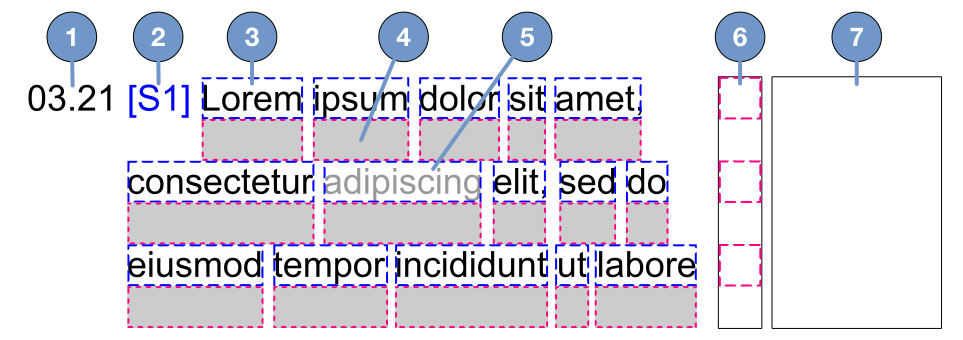
\includegraphics[width=\columnwidth]{figs/paper-interface-diagram.pdf}
  \caption{Diagram of the paper interface layout with timestamps at beginning of each paragraph (1), speaker
    diarization (2), word selection (3), word deletion (4), confidence shading (5), line selection (6) and a margin for
  freehand notes (7). Dotted lines indicate hidden active zones for selection (pink) and deletion (blue).}
  \label{fig:paper-interface-diagram}
\end{figure}

\begin{figure}[p]
  \centering
  \includegraphics[width=\columnwidth]{figs/paper-interface-example-annotations.png}
  \caption{Example of the paper interface system, with freehand annotations that demonstrate its use.}
  \label{fig:paper-interface-example}
\end{figure}

For each word in the transcript, two rectangular active zones are defined on the page -- one on the word itself and
another in the space directly below the word.  Any marks made on or below the word label that word as `deleted' and
`selected', respectively.  This allows the user to use a digital pen to delete words using a strikethrough, or to
select words by underlining.  The zone below is lightly shaded so that the user can see where the boundary lies between
the two regions.

For selection by drawing a line down the side, we opted to draw a long thin rectangle from the top to the bottom of the
page to the right of the transcript, rather than draw individual square boxes at the end of each line. We did this to
save some space, and to align with how the participants used the paper prototype.

The paper must be annotated using an Anoto Live Pen 2. This records the gestures made by the users digitally on the
pen.

To include audio editing functionality with the pen system, we integrated it with a screen-based interface. A diagram
of this integration is shown in Figure~\ref{fig:paper-screen-integration}. The screen
was used for asset management, including uploading new content and printing the transcript, and for viewing/changing
the edits made using the pen, and exporting the resulting audio or edit decision list.

When the pen is connected to its USB dock, the gestures are automatically uploaded to some Anoto software running
on the local computer, which processes the information from the pen. This is then sent to our server, which creates an
edited version of the transcript. This can then be accessed through the screen interface.

In addition to creating an edited version of the transcript, a PDF document of the transcript with the user's
annotations is created. This PDF can be viewed through the screen-based interface, so that they can refer to any notes
they made in the margins.

The user can export the audio from the edited transcript using the screen interface. Two types of export format are
supported. The user can download an EDL of the edits for either the SADiE or StarTrack audio editing systems.
Alternatively, they can download an edited version of the audio as a WAV file.

\begin{figure}[ht]
  \centering
  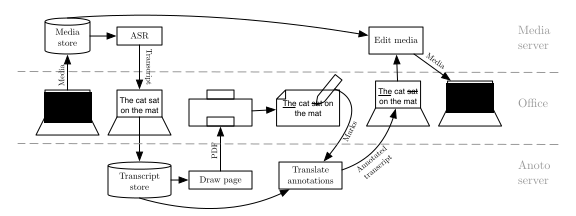
\includegraphics[width=0.5\columnwidth]{figs/uist-sys-diagram}
  \caption{Integration between the paper and screen interfaces, flowing from top to bottom.}
  \label{fig:paper-screen-integration}
\end{figure}

\subsection{Screen interface}
We updated the screen-based interface used in Chapter 5 to integrate the changes suggested by our findings. This gives
us something which we can compare the paper-based interface with.
The previous screen-based system is shown in Figure~\ref{fig:interface} on page \pageref{fig:interface}, and the
updated interface is shown in Figure~\ref{fig:dialogger-interface} on page \pageref{fig:dialogger-interface}.
The two major differences are that underline and strikethrough are used instead on drag-and-drop, and that only one
recording can be edited at any one time.

\subsubsection{Design decisions}

We replaced drag-and-drop with an underline/strikethrough method for three reasons.
Firstly, we found that there was not enough room to handle large clips, which was what most users were interested in.
Secondly, we found that users mostly used the tools for rough editing, so weren't as interested in mixing different
recordings together. This meant that we could concentrate on one file at a time.
Finally, we wanted the edit scheme to match our paper-based interface, as this would allow us to compare the two
modalities side-by-side.

There were many other smaller changes we made to the interface. We added double-speed playback to allow users to listen
faster than real-time, as requested by participant in our previous experiment. Previously, users could only make a
single edit per project. For the updated version, we allowed users to make multiple different edits of the same
recording by separating the original 'media' from the modified 'edits'. We also added a Save As button so that edits
could be branched.

We adjusted the speaker diarization display using a line down the side of each paragraph, coloured by gender and with a
label to the left to distinguish between speakers. We included confidence shading, but opted to use a dotted red
underline to indicate low confidence in order to match the style of word processors, and also to make it clearer.

\subsubsection{System description}

Users can login using their normal BBC account. They are then presented with the edit screen, which
has hidden sidebars on the left and right. Media that is uploaded is stored on the left-hand side, and any edits are
stored on the right-hand side. Edits can be exported either as an EDL or as an edited audio file. Users can only edit
one recording at a time, and multiple recordings must be mixed together at a later stage. Speakers are shown by a line
on the left of each paragraph, and any words with a low confidence are underlined with a dotted red line.

\begin{figure}[p]
  \centering
  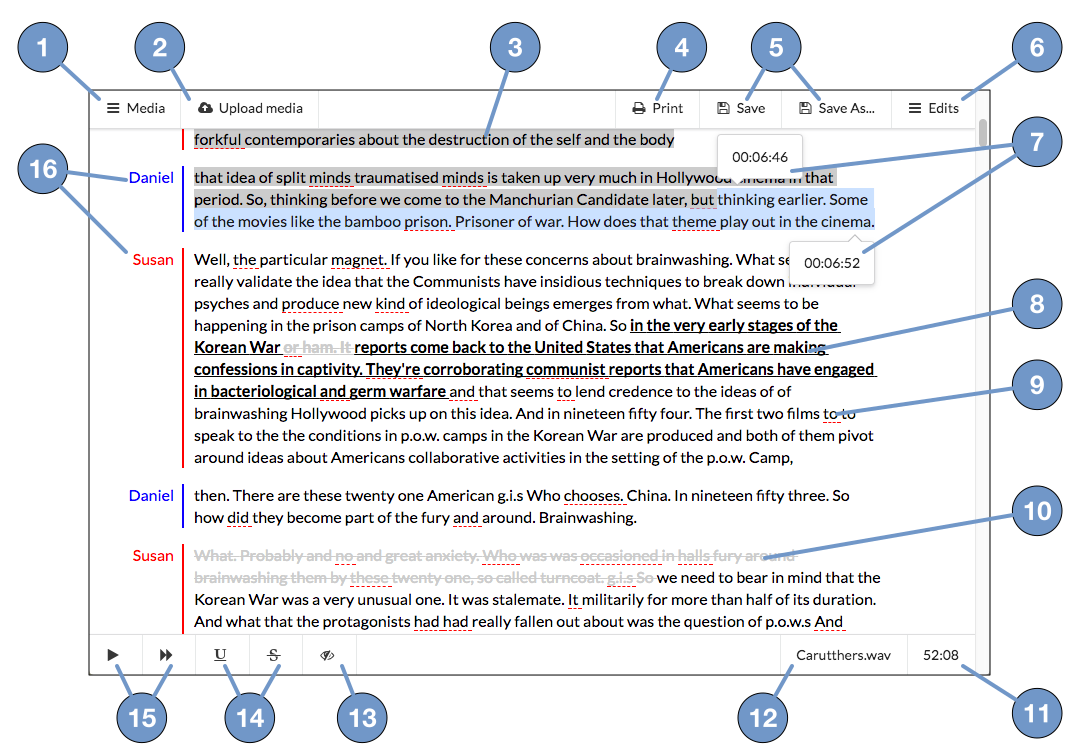
\includegraphics[width=\columnwidth]{figs/discourse-interface-labelled.pdf}
  \caption{Layout of the screen interface, which features 
    media storage (1),
    media upload (2),
    highlight of the current playback position (3),
    printing the transcript (4),
    saving edits and corrections to transcript (5),
    edit storage and export (6),
    displaying timestamps of the current selection (7),
    underlining words (8),
    confidence shading (9),
    strikethrough of words (10),
    display of edited audio duration (11),
    name of current asset (12),
    show/hide strikethrough (13),
    underline/strike buttons (14),
    playback buttons (15)
  and speaker diarization (16)}
  \label{fig:dialogger-interface}
\end{figure}

\begin{figure}[p]
  \centering
  \includegraphics[width=0.4\columnwidth]{figs/discourse-download-pdf.png}
  \caption{Close-up of the edits sidebar showing the button to export audio, and the option to download a PDF.}
  \label{fig:download-pdf}
\end{figure}

\section{Evaluation methodology}\label{sec:method}

To compare the paper and screen interfaces, we designed and conducted a user study.
The objective of our study was to 

\subsection{Design and procedure}
We ran a within-subjects user study in which we tested three different conditions: the pen interface, the screen
interface and a normal printed transcript. The printed transcript acted as a control, and was inactive in the sense
that it did not make use of the Anoto dot pattern technology.  The transcripts for all three conditions were generated
by the same speech-to-text system. In this study, we did not want to test the impact of the transcript itself, but
rather impact of the interface that is used to interact with the transcript.

We recruited professional radio producers exclusively from BBC Radio so that we could take advantage of the access that
was available to us. We recruited participants by sending an invitation by email to the current affairs, science and
documentaries teams in BBC Radio.  Through this, we recruited eight participants who had between 8 and 28 years
experience of professional radio production, with a mean average of 16 years experience.

%TODO Talk about length of recruitment, difficulty in completing study

We asked each participant to provide the audio recordings from three recent interviews they had made, so that the
content was genuine and fresh in their mind. We set a minimum duration of 20 minutes for each recording, as we found in
our previous study that there was no much advantage in using transcript-based editors for short recordings.

We divided our study into three stages, explained below:

\paragraph{Stage 1: Training}

Firstly, the participant was briefed on the study and asked to sign a consent form.  We then trained the
participant on the paper and screen interfaces using a test recording.  The experimenter explained all of the features
of the interfaces, and asked the participant to perform a sequence of actions based on a script. This allowed the
participant to use and experience all of the features for themselves. The participants were given the opportunity to
ask questions and play with each interface until they felt comfortable with how they worked and could be used.

\paragraph{Stage 2: Observation}

The second stage of the study was observing the participant edit three different recordings, each under one of the
three conditions.  The order of the conditions was counterbalanced to avoid carryover effects.  The tasks performed by
the participants overlapped with the work they needed to do already, which ensured that the tasks were genuine.  We
needed to use different recordings for each condition to ensure the tasks weren't just being repeated, but we asked the
participant to choose recordings from the same programme to ensure they were as similar as possible.

The observation took place at the participant's normal work environment, which in all cases was at their desk in an
open plan office. As the systems we built could be accessed using a web browser, the participant used their own
computer and desk. We considered recording the task using a video camera, but chose not to as we wanted to run the
study in the normal work environment. Due to the open-plan nature of the offices, this would have caused problems with
information security.

During the observation, the experimenter sat beside the participant and made written notes detailing what the
they were doing, and noting anything of interest. If the participant had any `down-time', the experimenter used this to
clarify anything they didn't understand. Items of interest included:

The specific items of interest at this stage include:
\begin{itemize}[noitemsep]
  \item Editing workflow
  \item Tools used
  \item Data generated
  \item Usability challenges and problems
  \item Navigation and edit actions
  \item Time taken to complete tasks
  \item Unexpected reactions
  \item Unanticipated usage
\end{itemize}

During each task, the experimenter kept track of how long it took the participant to complete the task, excluding any
time not spent on the task at hand (e.g. phone calls, making tea). We also logged the length of each recording being
edited.

%TODO What was the expected result?

After each task was completed, the experimenter asked the participant to fill out a questionnairre to measure the
usefulness and usability of the interface using Perceived Usefulness \citep{Davis1989}, shown in
Table~\ref{tab:usefulness}, and the Software Usability Scale \citep{Brooke1996}, shown in Table~\ref{tab:usability}.
Photographs were taken of the paper annotation and work environment, with the participant's permission.

\begin{table}
  {\small
    \begin{tabular}{ | l | }
      \hline
      Using this system in my job would enable me to accomplish tasks more quickly. \\ \hline
      Using this system would improve my job performance. \\ \hline
      Using this system in my job would increase my productivity. \\ \hline
      Using this system would enhance my effectiveness on the job. \\ \hline
      Using this system would make it easier to do my job. \\
      \hline
    \end{tabular}
  }
  \caption{Perceived usefulness questionnaire \citep{Davis1989}}
  \label{tab:usefulness}
\end{table}

\begin{table}
  {\small
    \begin{tabular}{ | l | }
      \hline
      I would find this system useful in my job. \\ \hline
      I think that I would like to use this system frequently. \\ \hline
      I found the system unnecessarily complex. \\ \hline
      I thought the system was easy to use. \\ \hline
      I think that I would need the support of a technical person to be able to use \\
      this system. \\ \hline
      I found the various functions in this system were well integrated. \\ \hline
      I thought there was too much inconsistency in this system. \\ \hline
      I would imagine that most people would learn to use this system very quickly. \\ \hline
      I found the system very cumbersome to use. \\ \hline
      I felt very confident using the system. \\ \hline
      I needed to learn a lot of things before I could get going with this system \\
      \hline
    \end{tabular}
  }
  \caption{Software usability scale questionnaire \citep{Brooke1996}}
  \label{tab:sus}
\end{table}

After completing all of the tasks, we asked the participant to fill out a form to measure user preference. The form
simply asked

\textit{``Of the three systems you have just tried, which of them would you most prefer to continue
using?''}

and had a checkbox for each of the three interfaces.

%TODO What is the expected result?

\paragraph{Stage 3: Interview}

For the final stage of the study, the experimenter performed a semi-structured interview with the participant. This
gave the participant the opportunity to discuss each of the three conditions in detail and compare them directly. An
audio recording was made of the interview, which was used to perform in-depth analysis.

We asked the participant the following questions:

{\singlespacing
  \begin{enumerate}
    \item Can you please describe your existing process for editing audio?
    \item What did you like or dislike about the paper-based system?
    \item What did you like or dislike about the screen-based system?
    \item What did you like or dislike about using normal paper?
    \item Overall, which of these systems would you most prefer to continue using, and why?
  \end{enumerate}
}

The first question was included to understand more about the participant's current approach, in case that affected
their preferences or usage of the systems.  The order of questions 2--4 were adjusted to match the order in which the
conditions were presented to the participant.  The final question was identical to that asked at the end of Stage 2, so
this gave the participant an opportunity to explain that decision.

\subsection{Analysis}

We performed both qualitative and quantitative analysis on the data we collected during our study.

For the qualitative analysis, we transcribed all of the audio recorded during the interviews by using our screen-based
interface to run speech-to-text and then correcting the words manually. This process produced 23,000 words of
transcripts. Using grounded theory, the principal investigator then openly coded the transcripts using the RQDA
software package. This produced 229 different codes. The principal investigator used mind-mapping software to group
these codes into 15 categories, then grouped the categories into three high-level themes. RQDA was also used to extract
representative quotes from the interviews to illustrate the points made.

During the study, we collected data about task duration, system preference, usefulness and usability.
We plotted the task duration measurements against the duration of the audio being edited. For each condition, we drew
the linear regression to see how the edit time is affected by longer or shorter recordings, and to compare the the edit
time of the three conditions.
The questionnaire data measuring the usefulness and usability were separately converted into scores between 0 and 100.
This follows the procedure described in \citet{Davis1989} for usefulness, and \citet{Brooke1996} for usability.
For the system preference data, we simply reported the count of the participants' preference for each system.

\section{Study results}\label{sec:paper-results}

In this section, we will present the qualitative results that emerged from the interviews with the participants,
followed by the quantitative data that we also collected.  The codes that resulted from the analysis of the interview
transcripts and observation notes are shown in Table~\ref{tab:paper-codes}. Three themes emerged from this coding
process -- `editing', `transcript' and `listening' -- and these are presented below individually. 

\begin{table}[h]
  \centering
  {\small
    \begin{tabular}{|l|l|l|} %p{0.18\linewidth}|p{0.2\linewidth}|p{0.5\linewidth}|}
      \hline
      \textbf{Theme} & \textbf{Category} & \textbf{\# codes} \\ \hline
      \multirow{8}{*}{Editing}
      & Collaboration & 15 \\ \cline{2-3} %Easier with digital representation (screen), Remotely, Compare notes with presenter, Timecodes or page/line numbers for reference, Side-by-side comparison, Google Docs, Share new material with presenter, With third-party institutions \\ \cline{2-3}
      & Annotation & 16 \\ \cline{2-3} %Colours, Highlight, Summary (auto?), Star, Labelling/numbering (auto?), Freehand, Speaker names, Music information \\ \cline{2-3}
      & Location & 11 \\ \cline{2-3} %Thinking space, Away from desk/screen, Downtime - plane/train/bus, Quieter, Concentration \\ \cline{2-3}
      & Export & 7 \\ \cline{2-3} %Transcript and annotations in DAW, Move selections to different track, Spaces between exported clips \\ \cline{2-3}
      & Pen & 35 \\ \cline{2-3} %Narrow margin, Could be lost/broken, No correction, Cost, Can't draw freehand, only strike/underline, Note digitisation, Poor ergonomics, Desired gestures, Simplicity/lack of functionality, Lack of undo (same as normal pen), Must be precise, Easier to edit without interrupting playback, Higher edit precision, Permanency increased decisiveness \\ \cline{2-3}
      & Technique & 24 \\ \cline{2-3} %Re-ordering and mixing (cut/paste), Pull out good bits, Remove bad bits, Rough edit first, Check nothing's been missed, Taking too much at early stage, Simultaneous correct and edit, Top and tail, Paper edit only (no listen), Multiple iterations (re-print) \\ \cline{2-3}
      & Decisions & 12 \\ \cline{2-3} %Must be made in real-time, Easier to decide with paper, Simultanous listening/editing easier on paper \\ \cline{2-3}
      & Interface & 21 \\ \hline %Familiarity, Learning curve, Auto-labelling?, Limited options (faster?), All in one place, Editing large chunks, Training/cheatsheet, One of many different systems \\ \hline
      \multirow{4}{*}{Transcript}
      & Paper & 15 \\ \cline{2-3}%Multiple windows/tabbing, Can't print on location, Quantity of paper (high), Takes time to print, Physicality, touch, Better, faster comprehension, Use of finger/pen to navigate, Bimodal reading/listening is better, Improves memory \\ \cline{2-3}
      & Accuracy & 17 \\ \cline{2-3} %Use of memory affects threshold, Field recordings, Affects speed, Punctation (distracting), Good enough, Speaker diarization, Affects amount of listening, Accents, Noise, Affects edit resolution, Doesn't show umms/breaths \\ \cline{2-3}
      & Generation & 10 \\ \cline{2-3} %Skipping/paraphrasing, Clerical job, Simultaneously making edit decisions in head, Takes too long, Third-party, overnight, Turnaround time, Question marks, Cumbersome/tedious \\ \cline{2-3}
      & Correction & 12 \\ \hline %Depends on length (don't need to for shorter), Not on paper, Fix repeat errors, For giving to other people, PasB transcript \\ \cline{2-3}
      % & Technique & TV (thumbnails, expense), Search archive material, Compare and orientate other recordings from programme \\ \hline
      \multirow{3}{*}{Listening}
      % & Speed & Discourse x2 playback hard to understand, Use memory to skip, Faster with transcript \\ \cline{2-3}
      & Navigation & 8 \\ \cline{2-3} %Can use finger as cursor on paper, Jumping around (easier with DAW), Timestamps, Reading ahead, Space bar to start/stop \\ \cline{2-3}
      & Criteria & 14 \\ \cline{2-3} %Intonation, Works on paper, not on audio, Transcript accuracy, Do clips work on their own/together?, Sound effects (e.g. thunder), Umms, Breaths, Does edit work?, Is transcript correct? \\ \cline{2-3}
      & Technique & 12 \\ \hline %Process/reinforce information, Fine editing, 'Listening is editing', Mental buffering during de-umming \\ \hline

    \end{tabular}
  }
  \caption{Themes, categories and number of codes that resulted from the quantitative analysis of the interviews and
  observations.}
  \label{tab:paper-codes}
\end{table}

\subsection{Editing}

\subsubsection{Edit technique}

% ITERATION

Participants reported that editing was an iterative process, not just a single stage.
The reason for iteration was that there are a number of unknowns when the producer starts editing.
Often if they are in the early stages of editing, they will not yet know which direction the programme is taking or
what the narrative will be, so are not sure which bits they should take.  This appears to affect the quantity of
material that is chosen.

\textit{``I was just taking probably taking far too much as I'm perhaps not quite sure what I need from that
interview.''} (P2)

% You might start off with one thought which was at the beginning of the interview and end with another thought in the
% middle of the interview somewhere else. You need to be able to do that to convey everything you've been speaking
% about in the interview. It's really not a matter of just taking three lines here, consecutive lines (P1)

% I think it is definitely Stage one. That's what I'm happy getting to using those techniques, and then. Then I want my
% filleted, but by no means final. Audio on the screen in front of me and then just to kind of muck about changing -
% there are things liek I wanted to change the order of some of the stuff in one of the interviews. I realised some of
% the stuff at the end needed to go further forward. But that's. that's for a later date (P4)

Choosing what to keep or not also depends on what was said in other interviews, and how much other usable material the
producer already has chosen. If they already have enough good material, then they know their standard for selection
will be higher than if they don't have enough.

% [My colleague] knows exactly what she wants straight away and can probably edit much faster than anyone else.
\textit{``Part of the editing is thinking what you want to keep in and thinking what will go with the rest of it. I
can't do that straight away, it takes several goes.''} (P8)

If they take too much, then they will have to reduce their selection down further at a later stage. If they don't take
enough, or take the wrong pieces, then they will have to go back to extend their selection or change it for a
difference piece.

\textit{``Usually when it comes to making the programme it will turn out that I want to use a clip in a different way;
  so I'll have to take the clip and add on a little bit, or get another piece from somewhere else that I wasn't
expecting''} (P1)

As they put the programme together, they will also have to reduce the programme down to a specific time. Radio
programmes must be edit to fit an exact time slot, so towards the later stages of editing, the producer must reduce
their selections to a specific time.

\textit{``For a documentary I would rough edit, put everything in order and edit once, edit twice and maybe a third
time to refine it, until you get it to time.''} (P8)

Throughout the editing process, the participants were making edit decisions. Some decisions are easier than others, so
many of the participants reported that they opted to perform a multi-stage edit, where the obvious edits are done
first, and the less obvious ones are done later. This then allows them to spend more time focussing on the most
difficult edits.

P1 also reported that they use transcripts to go back after editing to ensure that nothing important was missed in the
material they had not used.

\textit{``Sometimes I take a break from the screen and just have a look to check there's no crucial clips of bits of
audio I might want to use that I haven't put in the script.''} (P1)

P6 said they would have liked to perform multiple editing iterations using the pen interface, but were unable to using
the current design. They suggested that it may be possible to use different colour pens for each iteration, so that
they could be distinguished. For example, a red pen would show the edit gestures for the first iteration, blue for the
second etc. Implementing this would require an easy way for swapping the ink in the pen, which is currently not
possible without using tools.

% ROUGH EDIT
P1, P6 and P8 reported that the systems we tested were best suited to doing a rough edit as the first stage.  They used
the interfaces to get rid of the worst bits that they definitely weren't going to use, or to pull out the best bits
that they definitely were going to use.

\textit{``This paper edit stage is normally what I do just as a rough first thing to do. It's not for when I'm actually
editing the clips''} (P1)

We identified two reasons which may make the interfaces less useful for the later stages of editing -- re-ordering and
labelling.

% RE-ORDERING

After rough editing their material, the participants wanted to order their selections into a rough narrative to see and
hear how it would work. This is analagous to cut-and-paste in word processing, which many participants already use to
play around with re-arranging pieces of the transcript in their script. The interfaces we tested were designed for the
rough-edit stage, so did not allow the users to re-order content or mix content from different interviews. However,
there appeared to be an appetite for using the interfaces to go beyond the rough edit stage.

\textit{``Doing a cut which jumps from three different interviewees who are talking about the same topic that seems
like the next natural step''} (P3)

% LABELLING

In addition to selecting, removing and re-arranging their content, the participants were also interested in organising
their content.
Many participants did this by writing labels in the margins when using the normal paper or pen interface.

\textit{``I was labelling by summarising a paragraph in about two or three words, just who is speaking and the
substance of it''} (P5)

P3 suggested that it might be possible to automate this process using the text of the selected clip.

% I think the labelling thing would be. be something worth thinking about just so, because, especially as I've seen.
% Obviously, we don't have the audio but I've seen how you just get another cluster of audio. that that um that all
% looks. You know you're sort of almost starting again. And then you have to go back and look at the Look at
% the transcript. and say well which bit was this and which bit was that (P2)

\textit{``If it was to dump those separate clips in your [system] and name them according to the text, then that would
save twenty minutes suddenly in a single go.''} (P3)

% For instance, I'm doing the transcript was about Guantanamo and one was like okay there are three categories of
% prisoners and at one point I was quite tempted to be able to like label this. The whole thing. o.k. All audio
% could work for the forever prisoners and that other bit of audio... and that's in a way what you would do with SADiE
% or StarTrack You could kind of name your clips (P6)

\subsubsection{Edit decisions}\label{sec:paper-edit-decisions}

It is already known that reading from paper rather than a screen improves comprehension, but P4, P5 and P8 reported
that they could make editorial decisions faster and more easily on paper compared to the screen. The primary
reasons cited for this were the reduced fuctionality of the interface, uninterrupted playback of the audio and edit
gestures.

P4 reported that the limitations of the pen-based interface made the decision-making process faster. Without the
distractions of additional features such as correcting the transcript or navigating the audio, they were better able to
concentrate on deciding whether to keep or lose the piece of audio under consideration.

\textit{``Weirdly, I liked how it limited my options, because with the screen I think what slowed me down
  was the fact that I could be approaching it in different ways [by]
  %And so I was trying to approach it in several ways
  simultaneously correcting the transcript and trying to edit the content. [...]
  %and that's probably why it took as long.
  With the pen, I couldn't edit the transcript so there's no point stopping and [...]
  %also because I had a good
  %interviewee then I could just listen in real time. I knew roughly what I wanted him to say and 
  %I knew roughly where the good points were,
  so I could just listen through and then just go `no, yes, no, yes'.
I don't think I've ever done an edit that fast, where it was literally real time, so that was quite pleasing.''} (P4)

The screen interface we tested included integrated playback of the audio. Users could edit the transcript by using
their mouse to drag from the start to the end of their selection, and applying underline or strikethrough to mark the
words as selected or deleted. During playback, the audio would skip over any words marked as deleted.  If an edit was
made to the transcript during playback, this caused the playback system to pause while it calculated and applied the
audio edits.  The user had to manually restart the playback to keep listening.

By contrast, the pen interface did not include any integrated playback, so participants used a separate device to
replay the audio. This meant that the playback was not affected when any edits were made using the pen. Furthermore,
edits were made by drawing a line below or through the selection, which meant that the user could start to select or
delete words as they were listening, without knowing where they would stop.  P4 and P8 said that these differences
allowed them to edit as the audio played, in real time, without interruption.

\textit{``On the screen one, you're stopping and starting and it's slightly more cumbersome. I couldn't listen and edit
at the same time, whereas I could listen and edit with the pen.''} (P8)

Integrated playback is almost certainly a benefit, but interruptions to the playback risk slowing down the editing
process. However, this problem is technical and could be solved to allow uninterrupted playback while editing on screen.

%P7 felt that the pen system gave a different dynamic to the screen. They viewed the pen system as a way to make fast
%decisions on whether to keep or remove something.

%reading speed
P2 and P5 said they thought that they could process the information faster when reading on paper compared to the
screen.

\textit{``I think you do read slower on screen.''} (P2)

This aligns with the research by \cite{Kurniawan2001}, in which they compared the speed of reading from paper and
screens. They found that `in agreement with findings from previous studies, reading on paper was 10--30\% faster than
reading online'.  This would have helped them to keep up with the audio playback and allowed them to edit the content
in real time. With the screen, P5 found that they were selecting more audio than they needed because their inability to
keep up with the playback on the screen made it more difficult to decide.

\textit{``The [screen] just felt too quick and much much harder to make a decision. It was like `oh sod it just keep
everything', because you don't want to miss something.''} (P5)

% physicality, finger pointing
The ability to physically interact with the printed transcript may have also made it easier to follow than the
transcript on the screen. P5 talked about how they use their finger to follow their position on the paper. Although the
screen interface highlights the current playback position, the fact that it's being done for the user rather than by
the user may impact on their ability to process the information.

\textit{``I don't know why [the paper interface feels slower]. I wonder whether there's not a thing where
  you've got your finger being able to run along the line and hear it with your ears, whereas on the screen you're not
doing that in the same way. I'm not sure.''} (P5) 

The pen interface did not include any undo functionality, although the screen interface could be used to change the
edits at a later stage. Although writing with a pen on paper is already considered permanent, it is common to undo
mistake by scribbling out lines, for example. P3 and P6 said that they did not like that there wasn't any way to undo
the edits using the pen. P6 suggested that the lack of undo functionality may influence their editing process by
forcing them to be more decisive.

\textit{``It's harder to say `oh no I've changed my mind, I want to go back', so you almost have to be much more
decisive, which maybe is a good discipline.''} (P6)

%The participants in our study reported that having a transcript aided the edit decision-making process in several ways.
%It allowed them to save time by reading ahead and reading back.

%% READING AHEAD/BEHIND

%Having a transcript allowed participants to read ahead of their current listening position to see whether the material
%coming up was going to be of interest.  P2, P4, P5 and P7 talked about how they would read further down the page to see
%whether it was worth bothering to continue listening or not. This was used as a time saving tool, which would not be
%possible in an audio-only editing workflow.

%\textit{``You can glance at the transcript and just see that [...]
%%there's a paragraph of stuff that really is not really
%%relevant. Even though it's quite interesting. So you can glance down. See that summarise
%it's about a giraffe and you want stuff on a rhino and just discount it, whereas with your ears you've got to listen
%to the whole [thing]
%%whatever. So that's.
%That's where it was really helpful.''} (P5)

%Participants also reported using their memory of the interview to assist in working out how much they should skip.

%\textit{``It does save you time I think to when you are listening to and reading at the same time you think
%oh, I remember this stage of the interview. Absolutely useless. And so you just sort of go ahead a few pages and
%find where it got good again.''} (P2)

%% reading back
%Many participants talked about their motivation for navigating around the audio recordings while listening. P2 and P5
%talked about how they would hear something that would cause them to use the transcript to read what had happened
%previously to judge the relevance of what they had just heard.

%% keeping track of position
%P5 said the transcript helped them keep track of which interview they were currently editing. For a single programme,
%there will be multiple interviews recorded which has the potential to be confusing as to which interview the
%participant is currently editing.

%\textit{``Sometimes I do you know when you're doing three different programmes at the same time. Sometimes you can
%forget which one. You're on and so they're talking about revenge. but you're actually working a programme of
%forgiveness''} (P5)

%% FRESH IN MIND
%Making edit decisions is easier to do when the interview is fresh in memory, and most likely requires less
%re-listening. Therefore it is benefitial to start the editing process as soon after recording the audio as possible.

%% TOP/TAIL USING TRANSCRIPT
%TODO Move somewhere?
%Recordings of interviews will usually start before the interview begins, and end after the interview has concluded.
%Part of the rough editing process is removing the start and end of the recording, known as `top and tailing'. Some
%participants did this using just the transcript.

\subsubsection{Interface}

All of the systems we tested used the same transcription system, but presented the transcript to the participants
through different interfaces. When participants compared the systems, we did not find that there was any clear
`winner', but that the interfaces had strengths in different areas. The feedback we received from participants
indicated that the fuller functionality of the screen may make it better for more intensive editing, where producers
may not be sure what they want from a recording, while the more lightweight pen system may be better for quickly
selecting and removing content, when it is already known what is needed.

One of the frustrations expressed by participants about their current workflow was that they have to use multiple
different systems to put their programmes together. Often these systems have poor or zero integration, and the
interfaces have variations such as different keyboard shortcuts for the same task.

\textit{``We're darting in and out of five different systems a day, so we're editing in ProTools or writing emails or
doing this, and they've all got slight differentiations''} (P7)
%so sometimes you go 'oh, f*** it - I can't remember what it is I needed to do on that.

P3 and P6 said they enjoyed that the screen interface had all of the features available in the same place. The playback
of the audio was integrated into the interface, and they could correct and annotate the text, then export it without
having to use separate systems for audio playback or word processing. The pen interface did not support integrated
playback or correction while in use.

The lack of integrated audio playback and navigation in the pen interface made it difficult for participants to
interact with the audio content.  Although participants could use a separate playback device to navigate the audio,
they either had to do this `blind', or use the timestamps on the transcript to guide themselves to the desired
position. With the screen interface, participants could use the text to see where they were navigating to, making it
much easier to move around non-linearly.  We observed that when using the pen interface, many participants chose to
edit while listening straight-through, without navigating the audio at all.

The ease of navigation offered by the screen interface may make it better suited to editing recordings where producers
are more reliant on listening to the audio. This could include content with which the producer is less familiar, such
as a recording they were not present at, or a recording from the archive.

\textit{``I think if you're in a rush, and you know roughly what you've got, and it's an interview that's close to
  memory, you've done it that week, then the pen's really good. I think if you want to get into the guts of the interview
  and make sure they're actually saying something close to what they actually said, then you're going to want to work on
the screen.''} (P7)

%\textit{``It's a toss up between the two. They both have their merits in different scenarios I would say''} (P7)

%This may be due to the ease of navigating the audio in the screen interface, which is not present in the pen. This is
%because a separate device must be used for playback, and this is not linked to the words. This makes it more difficult
%to navigate non-linearly, which could be the reason for it being preferred for editing straight-through. Another reason
%could be because the pen interface has fewer features, so is seen as a more lightweight option against the feature-rich
%screen interface.

%% LEARNING CURVE

%There were mixed reports on the learning curve of using the screen. P3 thought that it was only a small step from word
%processing, but P7 and P8 thought there was a larger learning curve

%The learning curve for both interfaces was considered to be pretty short. P3 thought that the word processing style
%interface of the screen made it very familiar, but P8 found it tricky to get used to and P7 thought it could benefit
%from having some instructions.

\subsubsection{Location}

One of the findings from Chapter~\ref{chp:screen} was that the participants in that study struggled with working in
offices, so often worked away from their desk or at home. In this current study, many participants also reported that
their working environment affected their performance. Factors that influenced this included noise, their screen, their
desk and office distractions. P1, P5, P7 and P8 said that they often prefer to work away from the office, such as at
home, to help them focus and get more work done.

\textit{``I do go away from my desk. I find it useful to have thinking time away. [...] Sometimes I just like to have a
break from the screen.''} (P1)

P8 suggested that the pen interface was well-suited for travel, such as during commuting, which may provide an
opportunity to be productive in what would otherwise be considered downtime.

\textit{``I'd probably spend a couple of days at home to get it into shape [because] it's quieter [...]
  %. Not that this office is anywhere near as noisy as the last office. You can sort of get into a zone a bit,
  so you can really really concentrate. You save travelling time, and with the pen you could do stuff on the train [...]
  %couldn't you, because you can edit on a train. That would be more accurate... easier then editing on a train.
or on a bus. You could do it anywhere as long as it's not too bumpy.''} (P8)

P7 agreed, but thought that the screen interface would also work well. In either case, P7 said that noise-cancelling
headphones would be necessary so that the audio could be heard clearly.

Comfort was another factor that participants mentioned. P5 did not enjoy spending too long sitting upright at their
desk, and P7 cited comfort as a factor in where they prefer to work.

\textit{``I would say I feel more comfortable with a nice digital pen and a sheet of paper sitting on a couch or
  something like that. Doing it then realising it's cut the audio already... Christ, you could do it in bed - that would
really have your work-life balance sorted, wouldn't it?''} (P7)

\subsubsection{Pen}

This section discusses the pros and cons of the pen interface, as reported by the participants in our study.

% USER FRIENDLINESS

P5, P6 and P8 felt that the pen interface was user friendly, intuitive and simple. It closely replicates the existing
workflow of some producers and uses the same materials, which may have helped make some of the participants more
comfortable.

\textit{``It feels like you're working analogue, but you're actually working digitally. [...] It's nice to hold a pen
and go on real paper, which has the feel of every day life.''} (P7)
%\textit{``I do like a nice pen and paper I just do like to write stuff down and I'm quite scribbler.''} (P5)

% GESTURES

The design of our pen interface forced users to select or delete content by drawing lines within strictly defined
regions. The benefit of this design was that it was easily machine readable and could automatically edit the audio
accurately. However, the inflexibility of this approach meant that users could not freely draw on the page, other than
in the margin. P3, P5, P7 and P8 mentioned that they did not like having to draw within the fixed boundaries.

\textit{``[The pen interface] doesn't have the convenience of paper, which is that there's no real rules [and] you can
write anywhere on the paper.''} (P3)

In addition to restricting the gestures that users can make, the inflexibility of the system means that the gestures
are interpereted explicitly. P3 and P7 were concerned about potential errors that could be introduced if the lines they
were drawing strayed outside of these boundaries, which could lead to problems further down the line.

\textit{``If you're sloppy, then you're going to get a squiggle in the wrong area.''} (P7)

%P3 and P5 said that drawing in the boundaries would take some practice
%The underline area was shaded to help guide users as to
%where the boundaries were, but P8 found them to be too faint.

%P3 showed an interest in having more options for gestures to select or delete content, such as circling words or
%sentences of interest.

%TODO Examples of margin writing
We included a margin on the right side of our page layout to allow users to make freehand annotations. All of the
participants used margin to write labels about the content, and make notes for themselves. You can see examples of this
in Figure X. We did not attempt to digitise these notes, as this would require them to be written in a more structured
way. However, P3 would have like them to be transcribed and digitised along with the edits, as this would save them
having to do this manually afterwards.

%\textit{``you usually scribble in margin notes that go 'I don't need this, I need that' and 'where's this?'. Yeah, it's
%all part of the building block of the programme''} (P7)

% OTHER BENEFITS

%P7 liked the fact that it felt as though they were using an analogue workflow, but it was actually digitial.

% PRECISION

Participants could select words by underlining them, or select whole lines by drawing a line down the side. P5 thought
that using the line down the side was a faster way to edit the speech, and that the precision was sufficient for
doing a rough edit as they normally would.

P8 felt as though
the pen was more accurate than the screen. Although this is technically not the case, performing a physical underline
gesture may be less cumbersome than using the mouse to highlight the words on the screen.

P8 said they felt that the pen allowed them to be more precise than with the screen. This is technically not the case,
as both of them are accurate to the word level. However, the action of physically underlining the word rather
than using the mouse pointer to drag a selection might have felt more precise to them.

\textit{``[The pen felt] more accurate first time round and therefore maybe you only have to do two takes rather than
several. [...] You could get more precision I think.''} (P8)

One possible reason for this is because the pen can be used to draw a selection as the user is listening, but on the
screen, selection is a two-stage process where a button is pressed after the selection. Another possible reason is that
the participant may have been more comfortable with making the selection using a physical pen rather than a mouse
pointer.

% COST, SHARING

%\textit{``Presumably the pen is very expensive is it?''} (P2)

Participants had some concerns with practical issues about the pen system being used in the working environment.
Although the participants were not told how much the pens cost, P2, P5 and P7 showed concerns about the cost, which was
perceived to be a valuable item.  This gave rise to interest in what would happen should a pen go missing or get
broken, which was mentioned by P3, P5 and P7. 

\textit{``...not an issue until you lose the pen. You'll probably have to have it on a chain around your neck, like my
glasses nowadays.''} (P7)

A potential solution to the issue of cost is to share a pen amongst a number of producers in a team. This is
common practice with other bits of equipment like headphones and recorders. However, P3 and P5 noted that this already
causes issues where these shared items disappear or are not cared for appropriately.
%This has given rise to headphone being bolted to desks to ensure they don't get moved, for example.

\textit{``Pens which are not connected to anything will go missing and get lost.
  %umm so if that becomes part of your
  %standard workflow. is Everybody going to have their own pen? at the moment. We don't have a system where everyone has
  %their own headphones. This
  [We have a] constant problem with headphones going missing in this department [...]
  %which is a similar technology
and the solution for many desks is that the headphones are actually bolted down.''} (P3)

\subsubsection{Collaboration}

% PEOPLE

Producing a radio programme is not a purely solo effort and requires input from many other parties. Most
often, a producer will work with a presenter who is the voice of the show. They are usually involved in the
editing to some degree, depending on their level of interest and availability.

In addition to the presenter, the other people who may want to be involved in editing are assistant producers (although
this was not common amongst the producers we worked with), contributors to the programme and third parties, such as an
organisation that may have contributed to the production.

The involvement of other parties is usually to provide feedback on the edits the producer has made. Participants
reported that this is done in the form of sharing notes through a word processor or on paper, or having a meeting to
run through the current edit.

% TRANSCRIPT

P3, P6 and P7 said that using transcripts makes it easier to collaborate as it gives them a common reference point to
refer to.

\textit{``Obviously, working from transcripts makes it easier to compare notes and sort of work as a team''} (P6)

Text documents do not occupy must disk space, so can be transferred quickly and easily.
They can also be annotated without any specialist software. Audio recordings often take up a lot of storage and are
therefore more difficult to send to others. There is also not easy way for people to annotate audio recordings without
specialist software installed.

\textit{``Whoever the presenter is and myself - we would have heard some of it and then we decide together on paper. As
  they are writing the script, I'm editing the clips. I'm listening to it and sometimes I have to amend what we've
decided on paper because it doesn't quite work. There's a sort of back and forth going on.''} (P6)

% PAPER

Transcripts may be shared either on screen or on paper. When the people collaborating are in the same room, paper has a
number of advantages. Pagination can make it easier to point at something as the reference points do not scroll as they
do on screen. The physical nature of paper allows people to hand transcripts to one another.

\textit{``The way we're doing it is printing out our transcripts and we can all go `page fifteen' or you can
use timecodes, but there's a common reference, whereas if you're just doing audio it's harder.''} (P6)

However, when collaborators are not in the same physical space, sharing paper transcripts no longer makes sense.
Collaborating using screen-based transcripts is a powerful way to work with people remotely.

\textit{``Keeping it all on screen makes it much easier to share and be collaborative with people who are not in the
same room.''} (P3)

Services like Google Docs allow multiple users to work on the same document at the same time, even if they are on
opposite sides of the world. P6 reported that they already use Google Docs for this reason. However, currently the text
cannot be linked to media, so audio editing is unsupported. The same idea of collaborative simultaneous editing could
be applied to media, which would allow two people to compare notes and edit the audio at the same time.

\textit{``I think of the three, [the screen] has the most potential to be a collaborative thing. I'm not quite sure how
  it would work out yet. [...]
  %I don't know if you can share. and Everyone can compare versions.
  Maybe if you could have two scripts side by side to have my transcripts with my bits highlighted and the presenters,
with their bits highlighted.''} (P6)

As it is paper-based, the pen interface does not support collaboration outside of the same physical space. However,
it could still be used as part of the production, so long as it integrates with the collaborative tools.

\textit{``I would say in that case if you're sharing with your presenters or contributors or production staff, then
  you're going to be using the screen-based system. But you may have already used the pen to get to where you're
getting.''} (P7)

% LISTENING

With both paper and screen collaboration, listening is not often central to the process. Decisions are often entirely
based on the text. Integrating audio preview with a collaborative system may redress this balance by providing easy
access to the audio.

\subsubsection{Annotation}

%TODO P6 created a Box document to take notes

\begin{figure}[h]
  \centering
  \includegraphics[width=\columnwidth]{figs/pen-annotations-p5-cropped.jpg}
  \caption{Annotation by P5 in which the content is segmented using horizontal lines and labels in the margin. The
  middle segment is marked as removed using a diagonal line.}
  \label{fig:p5-annotations}
\end{figure}

% HIGHLIGHTER PEN

Participants used a variety of annotations as part of their editing workflow. Most used some form of highlighting to
select the parts they judged to be particularly good. Our system used an underline gesture to select words, but P1 and
P6 both suggested that they would prefer using a highlighter pen style mark.

\textit{``You did an underline, but I would like to have it as a highlighter pen as you've got that option on Word''}
(P1)

This would also mean that the transcript wouldn't have to be double-spaced, but it would require a system that can
distinguish between a strikethrough and highlight.

% MARKING SPECIAL REGIONS

P5 used annotation to mark up where the questions were in the interview. This allowed them to manually segment the
questions from the answers, which helped to structure the material. There was no formal method of doing this, but there
may be value in capturing this information in a structured way.

\textit{``I was just labelling by summarising a paragraph in about two or three words -- just who is speaking and the
substance of it -- or maybe just putting a cue to say that was a question.''} (P5) 

P7 said they were interested in including additional metadata like music reporting data. This is required when music is
included in a programme, so capturing this data in a structured way would save them having to complete and submit a
music reporting form.

\textit{``What I've started doing as a PasB information is adding in music details for post-production''} (P7)

% COLOURS

Participants used a variety of marks to rate the importance of their selections, including stars and astericies, which
we have seen previously. However, both P2 and P6 suggested using colours as a way of marking up different selections.

\textit{``Maybe if you had different colours you could do your first one in red [then]
  %and this was like kind of o.k. The first draft and you say okay, that I like. And then you'd go through it and somehow could
change the colour and underline it a second time.''} (P6)

Rather than using this just as a rating system (e.g. one is better than other), it could equally be used as a
categorial system for whatever context is needed for that producer.

\subsubsection{Export}

Both the screen and pen interfaces that we tested included a feature to export an edit decision list (EDL) of the
user's edits to a DAW. This allowed the participants to make changes to their edits using their existing tools, and to
integrate with their existing workflow.  P2 and P6 expressed frustration that annotations were not included in the
export.

\textit{``Once you have put it into SADiE you have to [label the content] again. It's almost like you've gone forwards
then you have to take half a step back and you lose a bit of momentum.''} (P2)

If user annotations could be captured in a structured way, then they could be used to label the clips that are exported
in the EDL.

The other frustration with the export feature was that in the EDL, the selected clips were all pushed together without
any gaps. P3, P5 and P6 said that they would like there to have been gaps between clips, so that it would be more
obvious where the edits are when listening back. When editing using the normal printed transcript, P5 and P8 moved
their selected clips to a different track (see Figure~\ref{fig:p5-screen}). This allowed them to see where the clips
were in the original recording.

\begin{figure}[h]
  \centering
  \includegraphics[width=\columnwidth]{figs/pen-screen-p5-lowres.jpg}
  \caption{P5 moved their selected clips to a separate track}
  \label{fig:p5-screen}
\end{figure}

%\textit{``With SADiE or StarTrack you could kind of name your clips. [...] If that could be done, that would help --
%that's the thing I missed.''} (P6)

\subsection{Transcript}

\subsubsection{Correction}

% NEED

The screen interface allowed users to correct words by editing the transcript. The normal paper allowed users to write
anywhere on the page, which could be used for correction, but the pen interface restricted users to writing in the
margin.  Five participants (P1, P2, P3, P4 and P7) corrected words while using the screen interface, compared to three
(P1, P2, P3) who made corrections on the normal printed transcript. The participants were unable to make corrections
using the pen interface, but P3 used the margin to write some corrections. 

Users are able to first correct the transcript using the screen interface before moving to the pen or printed
transcript.  This would change the workflow into a two-stage process of correction and editing, rather than a mixture
as it currently is. P3 said that they would rather do both tasks simultaneously.

\textit{``If I was given a magic pen and told to work this way I would end up doing a whole transcription correction
  process on the screen and probably just through impatience I would then start immediately selecting bits that
  are interesting for me. [...] I want to be able to do that all in one and I can't see a way of doing that with the
pen process at the moment.''} (P3)

Only one of the eight participants (P1) said that they wanted to correct all of the mistakes in the transcript. The
reason they gave for fully correcting the transcript at the beginning was that it would save time later on. However,
we observed that the rest of the participants chose only to correct errors that impacted on their ability to read the
transcript, or caused them to be distracted.

\textit{``It's good to have the option to sharpen it up as you go along because, obviously, reading back it'll slow
you down if it's completely the wrong word.''} (P2)

P7 said that fully correcting the transcript would only be necessary if the transcript was going to be
published, or if it was requested for legal reasons. They said that correcting the transcript amounted to nothing more
than pedantry, and was therefore an unnecessary part of the editing process.

\textit{``I would say [correction is necessary] only for a final transcript, or for a transcript that could have legal
  implications or factual implications where if the words are very wrong [...]
  %and you're trying to distribute that as some kind of material,
then it's going to create problems for you.''} (P7)

If the transcript is fully corrected at the start, then there is a risk that some of it will be immediately discarded,
whereas the decision to discard it could have been made without it being corrected.


% REPEAT ERRORS

Often, the speech-to-text system would make repeated mistakes on an unknown word that came up multiple times during the
interview. During our observation, this often occured with uncommon names of people that were mentioned in the
interview. P3 showed an interest in being able to correct these repeated errors efficiently, such as a find/replace
operation. However, the words were usually mistranscribed as a variety of different words, which makes the task more
complicated than a simple replacement.
%TODO Sugestions on what to do?

% PRIOR INFO

Correction only usually happens after the speech-to-text process has completed, but tying the correction process back
into the speech-to-text system may provide opportunities to improve the transcript quality.  P3 and P7 asked whether it
would be possible to provide some sort of custom training to the speech-to-text system to increase the accuracy for
their specific context. For example, if the producer informs the speech-to-text system about the topic of the
programme, then it could expand its vocabulary to include words related to that subject, or weight existing words as
being more likely to occur. This could also be used to assist the speech-to-text system in correctly transcribing the
names of contributors, or people mentioned in the interview, which would otherwise be unknown and therefore
mistranscribed.

\textit{``If you're doing a story about AIDS, there's going to be stuff about anti-retrovirals [...]
  %or something like that
  %and even in  quite mainstream subjects there is going to be some special vocabulary. Anyway, I just think that you
  %could. I'm just wondering. I can see that it would be a bit of extra trouble. But it seems like it's something that
The ability to teach it some words would be really good.''} (P3)

\subsubsection{Accuracy}

All of the systems we tested are based on speech-to-text and therefore impacted by the accuracy of the transcript.  The
speech-to-text system we used for this study was different to that used in Chapter~\ref{chp:screen}.  However, the
systems were both based on the same framework (Kaldi) so performed similarly, and the participants in this study
reported similar weaknesses to participants in the previous study.

All of the participants were successfully able to use the transcript to edit their material as part of the production
of their radio programme. All of the participants reported that the transcripts were sufficiently accurate for the
purpose of editing their content. Similarly to the study in Chapter~\ref{chp:screen}, the most common complaints were
of reduced accuracy due to heavy accents or background noise, and problems with speaker diarization and confidence
shading.

When we started the experiment, P7 had already been using a speech-to-text system to generate their transcripts. Based
on his experience, he reported that the accuracy of the transcript was affected by formality of speech, background
noise and accents.

\textit{``What we're finding these [speech-to-text] systems very useful for are for formal interview in well-spoken
English. What they're not good for is for informal interviews on-location with a lot of noise and heavy accents.''}
(P7)

% speaker diarization
As part of the transcription process, speaker diarization was used to estimate where in the recording different people
were speaking.  Our system over-guessed, so usually reported there to be more speakers than there actually were. It
also had occassional problems correctly identifying speaker gender. P2 and P3 reported that because of these problems,
they found that the speaker segmentation wasn't useful.

\textit{``[The speaker diarization] didn't seem to work at all at the moment, because not only was it saying there were
  lots of different people speaking when there was only two, but it often couldn't distinguish between a male and a
female voice.''} (P3)

% confidence shading
We used confidence shading to `low-light' words that the speech-to-text system was less sure of. This was designed to
make erroneous transcripts easier to read, by making the incorrect words less visible.  However, sometimes the
speech-to-text system gave a high confidence score to an incorrect word, or a low confidence score to a correct word.
This caused P3 to mistrust the confidence shading.

\textit{``The things it wasn't sure about weren't actually very often the real mistakes.''} (P3)

%The speech-to-text system also included a post-processing stage which punctuated the transcript. This was expected to
%make the transcript easier to read, but P4 reported that they found the errors in the punctuation distracting and were
%interested in correcting those mistakes. However, this was not mentioned by other participants.

% CONSEQUENCES

As part of their normal working practice, P6 uses perfect transcripts to guide them in the editing process. They
reported that the mistakes in the automated transcripts caused them to refer to the audio more often.

\textit{``I'm used to working with a transcript that is 100\% accurate, which means I don't have to go back to the
  audio as much. With [these systems], I had to go back to the audio more than I was used to, so I did feel that slowed
me down a little bit.''} (P6)

P2, P4 and P6 said that gross inaccuracies in the transcript distracted them, which caused them to read slower and
impacted the editing speed.

\textit{``Obviously reading back, it'll slow you down if it's completely the wrong word.''} (P2)

Erroneous transcripts may also cause producers to select more than is necessary, which would create more work for them
further down the line. P8 suggested that the accuracy of the transcript affected their confidence in making edit
decisions, causing them to make rougher edits than would otherwise be the case with a perfect transcript.

\textit{``The English was a bit confusing so I felt on that one, I could only do quite gross editing, topping and
tailing and taking chunks out.''} (P8)

P7 and P8 pointed out that because they can use their memory to make up for the mistakes in the transcript,
the transcript becomes less useful over time. This, in effect, gives automated transcripts a `shelf-life' of usefuless,
during which the producer can remember enough of the interview recording to make up for the inaccuracies. After a
while, the producer may need to correct the transcript before being able to use it.

\textit{``The fact that it wasn't very accurate in places made it difficult [partly because] it's been a long time
since I did those interviews. Normally it wouldn't be such a big break between recording and editing them.''} (P8)

\subsubsection{Transcript generation}

The participants in this study re-iterated what was said in Chapter~\ref{chp:screen} regarding their frustration with
manual transcription and the benefits of having the transcript automatically generated.  One of the participants (P7)
reported that they already make regular use of a commercial speech-to-text system called `VoiceBase' to automatically
generate transcripts. They said that in addition to saving them having to write it themselves, it also helped them to
share transcripts with third parties. P5 had previously tried a different commercial system called `Trint', but could
not continue due to the cost. None of the other participants reported as having used automatic transcripts as part of
their existing workflows.

P1 and P3 stated that they thought the automatic transcript itself was the largest benefit of the semantic speech
editing systems.  Although not stated as explicitly, the remaining participants suggested that the transcript
generation was a primary benefit of the systems we tested.

\textit{``The transcription thing is for me is eighty percent of the advantage.''} (P3)

P4 reported that they are normally not able to use a transcript due to time constraints. Access to affordable
speech-to-text would solve this problem.

\textit{``Almost all the time I don't have [a transcript] purely because it takes too much time to transcribe stuff.''}
(P4)

P8 stores the transcripts that they create because they sometimes find them to be useful later on. Ocassionally they
will go back to use parts of recordings they have made previously for their current programme.

\textit{``They're very useful to have and I always keep them. Quite often you might want them for a different reason.
  For that programme that we were doing today, I did a [similar] programme about four years ago, so I know where the log
is and I'll go back and take some chunks out of that.''} (P8)


% BENEFITS

%The transcript was also reported to make it easier to go back and find bits that were not originally selected, but were
%later needed, which also saved the participants having to re-listen to those bits.

%Most participants repeated that their normal process is to create transcripts manually, and that this is challenging,
%time consuming and takes a long time. Ocassiaonally a third party is used to transcribe overnight, but this is costly
%and normally unaffordable.

%P4 suggested that transcript were only necessary for recordings longer than 20 minutes, which supported our decision to
%restrict the study to longer recordings.

%P1 said that it was best to start transcribing as soon after the recording as possible, as it is much fresher in the
%mind. This may also apply to the editing process.

% EXISTING SPEECH-TO-TEXT USE


% TRANSCRIPT ITSELF


% TRANSLATION

P1 worked on programmes for the BBC World Service, which covers current affair stories around the world.  They often
have to deal with recordings of speech in foreign languages, which is especially tricky when they don't speak the
language. P1 said that their department spends money on translation services to help with this process. The recordings
are then normally sent to a colleague who can translate the audio, and provide a recorded translation of the parts the
producer is interested in using. These are then dubbed over the original recording. However, it can be difficult to
know where to position the translation over the original, as there are no timing references provided.

\textit{``This department doesn't realise how much money they spend on [...] the translation that we get done. I don't
know if you can do this in a different language?''} (P1)

Our speech-to-text process could be combined with automated translation to enable producers to navigate audio content
in their native language. There may also be scope to provide some level of editing capability, but due to differences
in word ordering (e.g. adjectives before/after nouns), the editing may only be possible at the sentence level. However,
the success of this is dependent on the accuracy of the translation, and P1 suggested this may require a good human
translator.

\textit{``I've had bad translators and just [gotten] gobbledygook as they've done a literal translation. I mean Google
Translate doesn't make any sense at all.''} (P1)

% DETECTING NON-SPEECH

The transcript did not include umms or breaths, but P7 and P8 showed an interest in being able to use the transcript to
de-umm the content. The speech-to-text system we used was trained to ignore umms and breaths, but sometimes they were
transcribed into various incorrect words.

\textit{``I think you could de-umm it very quickly, which is something we spend a lot of our time doing.  It's quite
funny working out what the umms were, because they are all sorts of different words.''} (P8)

Efficient de-umming would only really be possible if the speech-to-text system was explicitly trained to transcribe
umms and breaths, rather than attempting to ignore them.

\subsubsection{Paper}

% BENEFITS

Most participants commented that working with paper had a number of benefits to their workflow. P1, P2, P6 and P7 said
that it was easier on the eye and gave them a break from working on screen. P2, P5 and P8 said they found it easier to
read from paper than screen. P2, P5 and P7 enjoyed that paper was a physical, tangible medium which they could touch.

% memory
P8 reported that they found it easier to remember the content of the transcript when reading on paper rather than a
screen.  This aligns with the findings from \citet{Singer2017} in which students could recall key points and other
relevant information better from printed text than digital text.

%\textit{``I find it easier to read on on paper.''} (P2)

%\textit{``I much prefer to have paper. Even if I've got them on screen, [...]
%%. Um. I do use them on screen, but I.
%I do find the paper version easier.''} (P5)

%\textit{``If I've got a lengthy article, I won't even... well, I'll start off reading it on screen to check whether or
%not it's relevant, but then I'll just have to stop and print it.''} (P5)

\textit{``I find it easier to read off paper, and easier to remember stuff.''} (P8)

P1 thought that the paper interface allowed them to think more widely.

\textit{``It's essential to print. [...]
  %. I think I especially if you're doing the first thing with the SADiE
  %I like to have the transcripts printed out because at the moment how I work is
  I have the transcripts on my computer, but I still need to print them out to be able to edit because when I'm
  coming to write this script, I have to kind of think more widely. What bits am I going to put where? What's my
  structure? Where am I going to put this bit? Mentally, it is easier for me to refer to the [paper] transcript so
that I know where everything is.''} (P1)
%for when it comes to me actually using one of the bits. that I want


% ORIENTATION
P1 and P5 commented that using paper transcripts made it easier for them to orientate themselves. This is likely due to
the difference in technique for handling large bodies of text. Paper uses pagination to break the text up into fixed
chunks, wheras screen using a scrolling body of text. Scrolling interfaces have fewer points of reference, which can
make it difficult to orientate and navigate.
Screens have a limited amount of space in which to display the text, so use scrolling to display large amounts of text.
P1 and P7 were frustrated by the limited space offered by the screen, which caused them to have to 'flick through'
different windows.

\textit{``I think I just prefer to have a printed version. I find it kind of easier to have that to hand all the time,
rather than having to flick through screens all the time, back and forth through screens.''} (P1)

Paper can be arranged over a desk to help spatial navigation, and the page can be picked out and re-ordered, unlike
screen interfaces.
Physical paper also degrades subtely, and this could aid orientation.

\textit{``On the screen it's always the same quality, but [with] a fingered piece of paper [...]
  %can be a bit comforting as well.
you think, `this is not new to me', even if it feels new, I've been over this before.''} (P5)


% PRINTING AND WASTE

The physical nature of paper presents some well-understood challenges that are distinct from the screen interface.
Often transcripts can be very long, so printing them requires a large amount of paper. P2 used quite a long recording
for the experiment, which resulted in over 50 sheets of paper being printed. Although waste paper is recycled at the
BBC, it is still much more wasteful than using a screen interface.

\textit{``50 sheets of paper is rather a lot, yeah -- quite wasteful.''} (P2)

%P3 didn't like that the pen required a printer, and P5 was concerned about the waste caused by encoraging producers to
%use printed paper rather than screens.

% printer
Printing also requires access to a printer. This is not usually a problem in an office environment, but can be an issue
when travelling, or possibly when working at home, as the Anoto system requires a colour laser printer. However,
printing is not uncommon and colour laser printers are already commonplace within the BBC and other workplaces.

\subsection{Listening}

\subsubsection{Listening criteria}\label{sec:pen-listening-criteria}

%Although an edit may work well based on the transcript, it may not sound correct when you hear the audio. There are a
%number of reasons for this, and the participants were listening to the audio to try and avoid these situations.

We found in Chapter~\ref{chp:screen} that listening is an important part of the editing process, and so we are
interested to understand why it is so important. In this study, all of the participants chose to listen to the audio
while editing with the transcripts. In our interviews with the participants, they cited three reasons that listening
was necessary: processing information, judging quality and identifying non-speech sounds.

% DECISION MAKING

%Listening forms part of the decision-making process when editing. Many participants started editing their interviews
%without knowing what they wanted to use, or what direction their programme was going to take. The process of listening
%gave them the opportunity and the headspace to form those ideas and to make some of those edit decisions.

% PROCESSING 

% helps when can't follow transcript

P1, P4 and P6 reported that listening while editing made it easier for them to process the information that was
being communicated in the interviews.  P4 said that on its own, the transcript was only useful for making easier edit
decisions, such as `topping-and-tailing' where the informal discussions at the start and end of the recording are
removed.  When it came to making more complicated edit decisions related to reporting or storytelling, they found that
they needed to listen to the audio as the transcript was insufficient on its own.

\textit{``When it came to the bit where I needed to concentrate properly, I needed more than the transcription.''} (P4)

One practical benefit of combining listening and reading is that the mistakes in the transcript can be identified or 
ignored, depending on the goal.  P1 and P6 said this helped them to find where corrections needed to be made to the
transcript to make it readable for others. Also, as P1 pointed out, sometimes the transcript shows a word that is
actually inaudible or not present. Mistakes such as these need to be identified early on so that there is time to fix
them.

Beyond the practical benefit of knowing which words are correct, P2 and P8 suggested that the multi-modal input of
listening and reading helped them in understanding the content and making edit decisions.

\textit{``I think reading and listening at the same time makes it easier to take that amount of information on. It's
going into two sensory inputs so it's easier.''} (P8)

\textit{``It sort of reinforces what you're reading and vice versa.''} (P2)

%The benefits of multi-modal sensory input have been studied in previous work such as ABC, which found XYZ.

%All participants chose to listen to the audio whilst using the transcript. Section X discusses possible benefits of
%using a multimodal input, such as improved comprehension and retention. Participants also reported additional benefits
%of using the transcript and audio in combination.

% QUALITY

Another reason for listening is to judge the quality of the sound, which is not apparent from the transcript
alone. Although a transcript can tell you what was said, it does not tell you how it was said. This can change the
meaning of the words, and make the difference between an edit that works or does not work.

\textit{``I would like to hear the clips that I've underlined to know [...] how it sounds as a standalone clip, because
with some bits I started somewhere and ended somewhere else, so I wanna put them together.''} (P1)

%\textit{``I need to be able to [listen] at the same time because if I'm just doing it on the paper with the pen, I
%can't hear what they're saying. Most of the time it's not really the words, it's how they're saying it.''} (P1)

% intonation 
The direction of intonation (i.e. whether the voice rises or falls) can impact the suitability of a clip for an
edit. This is because the intonation of the end of a clip must match the beginning of the next clip, otherwise it will
be apparent to the listener that the two have been taken from different parts of a recording.

\textit{``It could be that I need another word somewhere or [...] the intonation is going up and it won't work as a
clip, so I need to hear it.''} (P1)

% poor quality 
As well as checking that the words were spoken in the right way, the participants were also looking out for any low
quality sounds that may not have appeared in the transcript. The two main offenders are `umm's and breaths.  Breaths
are a natural part of speech, but too much, too little or breaths which are too loud can be distracting to listeners.
Umms are also part of natural speech, but can reduce the intelligibility of the speech if there are too many.  The
speech-to-text system was designed to ignore these sounds, so they do not appear on the transcript.  It is therefore
usually not apparent that they exist without listening to the audio.

%\textit{``[The edit] might look all right there, and I know this is generally what they're saying here, but [...]
%%when it comes to actually getting that clip, I want to hear the clip So it's all right for a really rough. just
%%an idea. at a really early stage. But for me
%once you get onto an editing stage, even if it's a rough edit, I need to be able to hear it.''} (P1)

% NON-SPEECH

Finally, the participants were also interested in identifying non-speech sounds. Although speech-based radio programmes
are primarily concerned with voice, they are often mixed in with environmental sounds and music to enrich the listening
experience. Some producers even prefer to conduct their interviews outside of recording studios, as it can give the
programme more life. However, this could cause problems with speech-to-text systems and make it more difficult to edit
together later.

%\textit{``If I was making a heavily actuality-led programme, I wouldn't bother with those sort of transcripts, because
%what you want is the sense of the sound, of its audio environment.''} (P7)

\textit{``It would have been interesting to have done this with a project where you need to be listening for very
  different things. [I wonder] whether one could mark up on the transcript `atmosphere change here', `big rain cloud
there', `thunderstorm here', because you need to know where they are.''} (P7)

The speech-to-text process does not attempt to transcribe non-speech sounds. This means that producers must listen to
identify any sound effects or environmental sounds that might have occured during recording. In many cases, they may
want to seek these out to include in the programme, however this currently must be done manually through annotation.

\subsubsection{Listening technique}

In section~\ref{sec:pen-listening-criteria}, we discussed why the participants needed to listen to the audio. In this
section, we discuss how listening is used as part of the editing process.

% AUDIO-ONLY EDITING

There are a number of situations in which participants said they would edit using the audio alone. P4, P6, P7 and P8
all said that they sometimes edit without any form of supplementary material, using only the audio itself. When
the audio recording being edited is short enough that the producer can remember what was said and where, then
there is less need for a transcript. P4 put the cut-off threshold somewhere between 15 and 25 minutes.

\textit{``[Transcripts are] good to have a if you've got a long interview. I think for interviews that are under
  15 minutes, it's not. I can hold the whole thing in my head. [...] For things that are over 25 [minutes], then that's
when it starts to become useful.''} (P4)

P7 said that deciding whether to use transcripts depended on the type of programme being made. Studio recordings of
speech contain no other sounds except the speech, so they get their meaning purely from what is said and how it is
said. Some other programmes focus more on the auditory experience by using field recordings, sound effects and music.
In these cases, there may be little benefit in using transcripts at all.

\textit{``If I was making a heavily actuality-led programme, I wouldn't bother with those sort of transcripts because
what you want is the sense of the sound, of its audio environment.''} (P7)

%P8 reported that they stop using their transcript once they have completed a rough edit of their material. This
%may be that the quantity of material has been reduced enough that there is more benefit in making decisions based on
%the sound rather than the meaning of what is being said.

%P6 suggested that audio-only editing is not necessarily better or worse than semantic editing, but that it in
%alternative that may be useful in some situations.

% RE-LISTENING

P1 and P7 reported that their existing editing workflow often involves re-listening to the material they recorded in
full.

\textit{``I would go through every single interview and listen through it, from beginning to end.''} (P1)

They reported that this allows them to refresh their memory, and to start making decisions on what to lose or to keep.
P2 said that they found manual transcription to be a good opportunity to re-listen to material for similar
reasons.

\textit{``Logging is good in some ways in terms of the process -- you sit, you listen back, you write it down, you
underline your key bits -- but it's also a clerical thing that takes a lot of time, which we don't really have.''} (P2)

Although removing the requirement to manually transcribe recordings reduces the burden on producers, there is a risk
that it takes away the opportunity to re-listen to material. This may introduce an unintended negative impact in that
edit decisions are based more on the words that were spoken and less on how the sound and auditory experience.

% THINKING/BUFFERING

In the existing workflow, P7 de-ummed the audio as they listened to it. They reported that they did so because, for
them, de-umming performed a similar function to `umm'ing itself, in that it gave their mind an opportunity to buffer.
This helps them to process and retain the information they are hearing.

\textit{```Umming' is a way of the mind buffering and `de-umming' is also a way of the mind buffering whilst you edit.
You waste 45 seconds or whatever on a de-umm, but you don't actually waste it as you're listening to the audio.''} (P7)

\subsubsection{Listening navigation}

P4 talked about how they used the timestamps written on the page to navigate forwards or backwards. This is a step up
from their existing workflow where they have to do this without the timestamps. However, they pointed out that this
would be much simpler if the audio could be navigated using the pen interface.

P2 also reported that they used their memory to skip parts that they remembered were not worth using.

\subsection{Metrics}

% Preference
\subsubsection{Preference}

Directly after each participant completed the three tasks, we asked them to select which of the interfaces they would
prefer to continue using. As shown in Figure~\ref{fig:preference}, four of the eight participants chose the pen
interface, with two (P3 and P6) choosing the screen and two (P1 and P4) choosing the normal paper transcript.

Although we expected participants to be split between the paper and screen interfaces, we did not expect anybody to
prefer the normal transcript, as it did not include any semantic editing functionality.  Both P1 and P4 preferred the
normal paper transcript because it allowed them to continue to use their existing workflow, which they found easiest
and most comfortable.

\textit{``I can retro fit it into the way that I currently work most easily because it is essentially the same way that
I do work, but with an extra paper transcript.''} (P4)

\textit{``That is the most natural to me that is what I felt most comfortable with doing.''} (P1)

The paper transcript allowed participants to use their existing tools, which they used regularly, and therefore could
achieve the same objective without having to learn how to use new systems or interfaces. Although the normal printed
transcripts did not include any features other than the transcript itself, the fact that two of the producers would
prefer to use it demonstrates the value of the transcript itself and the familiarity with the toolset.

\begin{figure}[p]
  \begin{subfigure}[b]{0.5\textwidth}
    \centering
    \resizebox{\linewidth}{!}{
      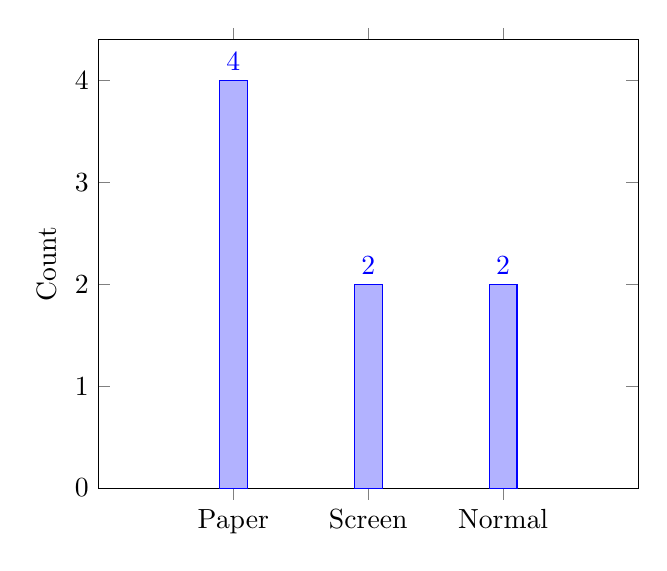
\begin{tikzpicture}
        \begin{axis}[
          ybar,
          ymin=0,
          enlarge x limits=0.5,
          legend style={at={(0.5,-0.15)},anchor=north,legend columns=-1},
          ylabel={Count},
          symbolic x coords={Paper, Screen, Normal},
          xtick=data,
          nodes near coords,
          ]
          \addplot coordinates {(Paper,4) (Screen,2) (Normal,2)};
        \end{axis}
      \end{tikzpicture}
    }
    \label{fig:preference}
    \caption{System preference}
  \end{subfigure}
  ~
  \begin{subfigure}[b]{0.5\textwidth}
    \centering
    \resizebox{\linewidth}{!}{
      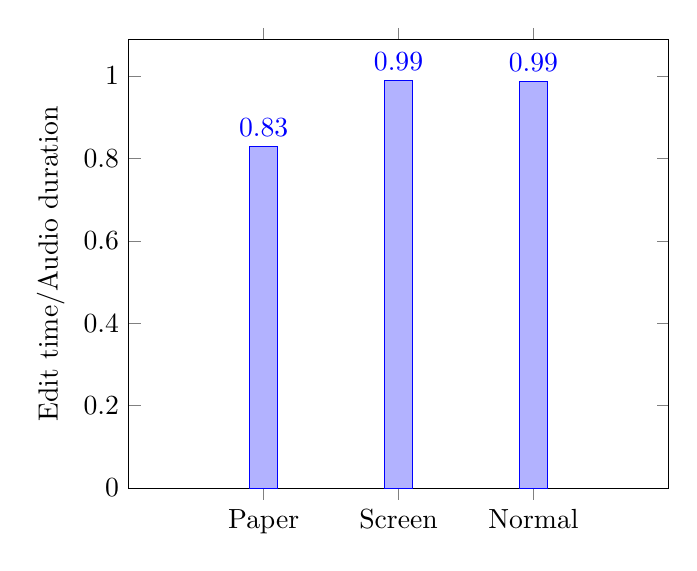
\begin{tikzpicture}
        \begin{axis}[
          ybar,
          ymin=0,
          enlarge x limits=0.5,
          legend style={at={(0.5,-0.15)},anchor=north,legend columns=-1},
          ylabel={Edit time/Audio duration},
          symbolic x coords={Paper, Screen, Normal},
          xtick=data,
          nodes near coords,
          ]
          \addplot coordinates {(Paper,0.8295) (Screen,0.9890) (Normal,0.9867)};
        \end{axis}
      \end{tikzpicture}
    }
    \label{fig:paperspeed}
    \caption{Mean edit time, relative to the duration of the audio being edited. There is no statistically significant
    difference between the times.}
  \end{subfigure}
  \caption{Comparison of metrics}
\end{figure}

% Usefulness and usability
\subsubsection{Usefulness and usability}

\begin{figure}[p]
  \centering
  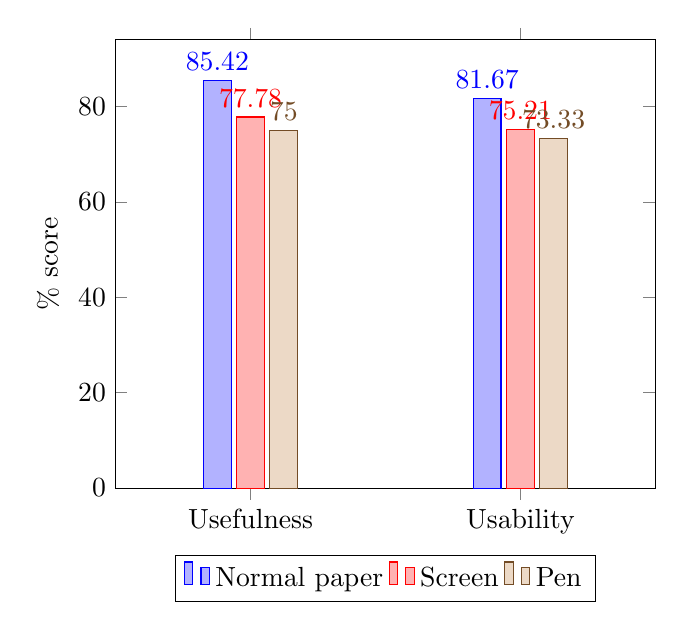
\begin{tikzpicture}
    \begin{axis}[
      ybar,
      ymin=0,
      enlarge x limits=0.5,
      legend style={at={(0.5,-0.15)},anchor=north,legend columns=-1},
      ylabel={\% score},
      symbolic x coords={Usefulness, Usability},
      xtick=data,
      nodes near coords,
      nodes near coords align={vertical},
      ]
      \addplot coordinates {(Usefulness,85.42) (Usability,81.67)};
      \addplot coordinates {(Usefulness,77.78) (Usability,75.21)};
      \addplot coordinates {(Usefulness,75.00) (Usability,73.33)};
      \legend{Normal paper, Screen, Pen}
    \end{axis}
  \end{tikzpicture}
  \label{fig:usefulusable}
  \caption{Mean average scores for usefulness and usability. There is no statistically significant difference between
  the scores.}
\end{figure}

% calculated using http://www.statisticslectures.com/calculators/anovawithin/index.php
Figure~\ref{fig:usefulusable} shows the mean average scores of the usefulness and usability of the three systems.  We
performed one-way within-subjects ANOVA on the usefulness and usabilty scores. This found that there were no
statistically significant differences between the three systems for usefulness [$F(2,14)=0.788, p>0.05$], nor usability
[$F(2,14)=1.068, p>0.05$].

We can compare the usability of our three systems to other systems in general by using the SUS scores from 
previous studies. These have been collected and reviewed in \citet{Sauro2016}, which also includes method to convert
the SUS score into a representative grade between A and F.  The grades for normal, screen and pen were A, B and B--,
respectively. This shows that, generally speaking, the tools seem to work well.

Although there was no statistically significant difference, the higher scores received by the normal printed transcript
are concerning. This could imply that the semantic editing features offered by the screen and pen interfaces have a
negative impact on the usefulness and usability of the system. However, it is also possible that participants scored
the normal paper system higher as they felt more comfortable and familiar using their normal toolset rather than a
prototype.

%Several participants felt as though the existing workflow was the most comfortable or easiest of the three conditions
%we tested. P7 said that having a printed transcript was useful as an aide memoire.

%\textit{``what I liked [about the normal paper] is that it's very similar to what I'm used to so there is familiarity''}
%(P6)

%Some participants preferred the normal printer paper transcript to either of the semantic editing interfaces, as it was
%more familiar to them.

% Speed
\subsubsection{Speed}

%\begin{figure}[p]
%\centering
%\begin{tikzpicture}
%\begin{axis}[
%legend pos=outer north east,
%legend cell align=left,
%xmin=0,
%ymin=0,
%xlabel={Audio length (mins)},
%ylabel={Edit time (mins)}]

%% NORMAL
%\pgfplotstableread{
%X Y
%30 30
%58 43
%32 23
%35 53
%28 35
%28 32
%47 62
%28 22
%}\normaltimes
%\addplot [only marks, mark = *, red] table {\normaltimes};
%\addlegendentry{Normal paper}
%\addplot [thick, red, forget plot] table[
%y={create col/linear regression={y=Y}}
%]{\normaltimes};
%%\addlegendentry{Normal trend}

%% SCREEN
%\pgfplotstableread{
%X Y
%37 24
%61 61
%30 30
%25 49
%26 31
%41 28
%37 37
%33 45
%}\screentimes
%\addplot [only marks, mark = square*, blue] table {\screentimes};
%\addlegendentry{Screen}
%\addplot [thick, dotted, blue, forget plot] table[
%y={create col/linear regression={y=Y}}
%]{\screentimes};
%%\addlegendentry{Screen trend}

%% PEN
%\pgfplotstableread{
%X Y
%12 9
%75 56
%31 17
%22 19
%27 27
%38 37
%33 33
%28 41
%}\pentimes
%\addplot [only marks, mark = diamond*, green] table {\pentimes};
%\addlegendentry{Pen}
%\addplot [thick, loosely dashed, green, forget plot] table[
%y={create col/linear regression={y=Y}}
%]{\pentimes};
%%\addlegendentry{Pen trend}

%\end{axis}
%\end{tikzpicture}
%\caption{Edit time performance for each editing system, with linear regression plot}
%\label{fig:penedittime}
%\end{figure}

We measured the time it took for the participants to complete each of their editing tasks during the experiment.
Longer audio files take longer to edit, so we also measured the the duration of the original audio recording that they
used. We then divided the edit time by the audio duration to produce the relative edit time.

%The mean edit time per minute of input audio was 59.2, 59.34 and 49.77 seconds for the normal paper, screen and pen
%interfaces, respectively.

% calculated using http://www.statisticslectures.com/calculators/anovawithin/index.php
The mean average of the relative edit time for each system is shown in Figure~\ref{fig:paperspeed}. We performed
one-way within-subjects ANOVA on the relative edit time and did not find any statistically significant difference
[$F(2,14) = 0.931, p > 0.05$], which may be due to the small sample size.

The screen and normal paper interfaces had the same mean relative edit time, but the pen was faster by 16\%.  This was
surprising, as we expected the screen interface to be faster than both the pen and normal paper due to its more
powerful navigation features. As discussed in Section~\ref{sec:paper-edit-decisions}, some participants found that the
simplicity of the pen interface allowed them to make edit decisions faster. This matches with the data, but the results
are not statistically significant so more investigation is required.

\section{Discussion}\label{sec:paper-discussion}

%In this chapter, we were interested in exploring the relative benefits of semantic editing of speech using a pen-based 
%interface, compared to a screen-based interface.
%We found that the behaviour of participants was different between the pen and screen. With the pen interface,
%participants make quick decisions on selecting or removing content, while with the screen, they corrected some words
%and navigated the audio to make more considered decisions. The screen interface allowed participant to correct the
%transcript while they edited, giving them a richer output, while the pen did not.


%There was no integration between the pen interface and audio playback. Although this did not prevent the participants
%from navigating the audio, many did not do so, which meant that they edited the audio straight through in real-time. 
%The pen interface also did not include any functionality for correcting mistakes in the transcript. Although this meant
%that the mistakes were still present after editing, the participants were not distracted by making corrections, so they
%could get on with making edit decisions.

%In their interviews, participants talked about the benefits of using paper. It is already known that reading from paper
%rather than from a screen allows readers to gain a deeper understanding, cross-reference and interleave reading and
%writing.  The comments made by participants suggest that these finding also seem to apply to semantic speech editing on
%paper. Additionally, there were some suggestions that it may be easier to listen and annotate simultaneously, and
%easier to make edit decisions when using paper.

%There are a number of improvements that could be make to the pen interface, which may have caused it to be rated as
%less usable and useful than the other systems we tested. One of the main benefits of working on
%paper is that it can be annotated freely. However, the system we used to build our prototype forced users to draw only
%within a margin, and to edit by drawing strictly within defined borders. This caused many participants to be concerned
%about introducing errors by drawing outside of the lines, and did also not like not being able to draw freely.
%Future systems should consider using a more advanced system that takes a less literal approach to annotations.

%The screen interface added two features over the pen interface -- integrated playback and correction. The ability to
%navigate the audio playback using the transcript allowed the participants to skip forwards and backwards easily
%without having to use timestamps. This lowered the barrier to replaying content that was of interest, or reading ahead
%in the transcript and skipping over content that was not of interest.

%In the screen interface, the transcript could be corrected while editing. With the pen interface, correction was not
%possible on paper, but could be done using the screen interface before printing it out.


%PEN
% most popular, fastest, but rated least usable and useful
% simplicity and lack of navigation/correction may have led to increased speed
% lack of integration with listening may have led participants to use interface differently from screen
% participants talked about benefits of using paper - easier to read, remember, make decisions, orientation
% did not include correction or detect written notes
% strictness of gesture detection has potential to introduce errors

% SCREEN
% included correction, participants mised correction with editing
% distraction of correction may have slowed edit time
% ease of navigation makes it more suitable for exploring content, experimenting

% NORMAL
% Quarter of participants didn't want to continue using semantic editor
% Familiarity, reliability are important when workflows are tight

\subsection{Editing}

%Editing is a multi-stage process. Participants said that the interfaces we tested were best suited to the first rough
%editing stage. This may be due to lack of features for organising and re-ordering content. We addressed this by
%integrating with DAWs, but the transcripts are lost through this process. Adding features for labelling and re-ordering
%would allow users to use transcripts for the later stages of editing.

Through our study, we wanted to learn how professional radio producers were impacted when performing semantic speech
editing using a pen-based interface compared to a screen-based interface.  We found that neither interface was best in
all situations, but that each was better suited to different uses and circumstances.  Broadly speaking, we found that
our pen interface was better for making simple edits involving quick decisions, using familiar content with a
high-quality transcript, for producers working away from their desk, or with others in the same room.  By contrast, we
found that our screen interface was better suited to more complicated editing involving complex decisions, using less
familiar content with a lower accuracy transcript, for producers working at their desk, or with other people remotely.

Three of the participants reported that they could edit faster and more easily using the pen interface compared to the
screen.
%Additionally, the mean relative edit time of the pen was faster than the screen, but this was not statistically
%significant.
We found that this may have been partially due to the faster reading speed of paper and the more natural edit gesture
of the pen, and partially due to the lack of integrated playback and correction features.  This reduced functionality
caused participants to focus more on the editing task at hand, rather than being distracted by correcting or navigating
the transcript.

% integrated playback and correction
The screen interface included integrated playback and correction, which made it a more powerful tool.  P7 reported that
this made it suitable for more challenging editing tasks or exploring less familiar content, where the producer needs
to be able to listen and navigate efficiently. The integrated listening also made it better for working with less
familiar or lower accuracy transcripts as participants could tolerate the errors by using their memory of what was
said, by listening or by correcting the errors. The screen makes it easier to listen and correct the errors, so is a
better choice for editing less familiar content or lower quality transcript. 

% collaboration
Producers do not work alone and need to collaborate with others during production. The physical nature of paper made
the pen interface suitable for working with others in the same room, as it allowed them to work around a desk,
spatially arrange the pages and refer to the transcript by pointing. However, this also makes it impossible for the pen
interface to be used remotely. The digital nature of the screen interface makes it easy to work with remote
collaborators. There is also potential to extend the interface to use operatial transformation, which would allow
multiple users to edit the same content simultaneously.

% portability
Half of the participants reported that they like to work away from their desk or office as it helps them to focus. Pen and
paper is naturally very portable and can be used almost anywhere. As it is does not use a screen, it is smaller,
lighter, easier on the eyes and has a longer battery life. Several participants reported that this makes it more
suitable for travel, and would allow them to work in more comfortable places. However, the requirement to print the
transcripts makes it unsuitable for working on the road. By using a laptop or tablet, the screen interface is also
portable. The screen also include the advantages of integrated playback and correction, and could be used on the road
as it doesn't need a printer.

% improvements
Our study identified a number of improvements that could be made to the pen and screen interfaces. Three participants
reported that the interfaces could currently only be used for rough editing as they lacked features for labelling or
re-ordering material. For the pen interface, handwriting recognition could be used to label a specified region, or the
nearest selected content. Two participants requested that the labels should be included in the exported EDL, so that
they would integrate with their existing tools. Two other participants said they would prefer to use a highlighter pen
than to underline, and others suggested using multiple ink colours to label content or to indicate multiple iterations.
However, we are not aware of any digital pens that support highlighting or quickly swapping nibs.

% implementation constraints
Our choice of technology for implementing the pen interface introduced some constraints that affected our design.
Users edited the content by underlining or striking text within a set of rectangular boxes. There were interpreted
literally, which created a potential source of errors, and forced the participants to draw carefully. This design also
prevented us from including correction and undo features, and the batch-mode operation of the pen prevented us from
including integrated playback.  By overcoming the constraints of our implementation, a pen interface with integrated
listening, correction and undo could be created. We expect that this would allow users to combine the benefits of
working with paper with the full feature-set of the screen interface. However, there is also a risk that by adding more
features to the pen interface, the benefits of its simplicity would be lost.

%As humans are not
%good at drawing straight lines in freehand, it would be better to create a system that was more forgiving in this
%respect.

Electronic paper may provide the technical solution that could bypass these constraints. At the time we developed
our pen interface, there were no e-paper devices that supported digital ink interaction, but these will become
available in the near future.  For example, the reMarkable tablet\footnote{\url{https://remarkable.com/}} is an e-paper
device with a digital ink interface that will be available in late 2017. Although e-paper displays do not seem to
currently match paper for reading speed, comprehenson or eye fatigue, they are likely to improve over time and may
provide a good middle-ground between paper-based and screen-based systems. 

The quantatative data we collected did not produce any statistically significant results and produced very mixed
messages. On the one hand, half of the participants selected the pen interface as the system they would prefer to
continue using, and it had the fastest mean relative edit time. However, the participants also rated the pen interface
as the least usable and least useful of the three.  Despite it having no semantic editing capability, the participants
rated the normal paper interface as most usable and useful, and a quarter selected it as the preferred option.
Based on this data, it is not possible to draw any conclusions.

\subsection{Transcripts}

All of the participants were able to use the automated transcript to edit speech recordings for their radio programme,
supporting what we found in Chapter~\ref{chp:screen}. One of the participants in this study had already started using
speech-to-text as part of their normal workflow. As automated transcription becomes more widely available, it is
important to design tools that make the best use of the extra information.

As the semantic editing tools we tested are based around transcripts, the accuracy of the transcript has a direct
effect on the performance and usage of the tools. We identified five different areas that were affected by transcript
accuracy: correction, reading speed, reliance on listening, longevity and edit granularity.

% correction, reading speed
Clearly, the more errors that occur, the more likely it is that corrections will be needed. However, the vast majority
of participants were only interested in correcting mistakes that were distracting and impacted their ability to read
the transcript. Three participants reported that these distractions slowed down their reading speed.  For the most
part, full correction is only needed if the transcript is to be published or is required for legal reasons. Publication
of transcripts is not yet required, but doing so would make radio programmes more easily discoverable and searchable.

%This is similar to \citet{Ranjan2006}, which found that search time falls as the accuracy increases.

The speech-to-text system we used often mistranscribed unknown words into a variety of different words, which means
they must all be corrected individually. This usually occured with words specific to the programme, such as names of
contributors. To avoid this, unknown words could be added to the dictionary of the speech-to-text system prior to
transcription. By providing additional contextual information, such as the programme topic or number of speakers, the
transcription system could improve the transcript accuracy by using this to better calculate the likelihood of a given
word occuring or limiting the number of unique speaker segments.

Two participants showed an interest in using semantic editing to remove `umm's and breaths. The speech-to-text system
we used was not designed to detect and transcribe these noises. As with other unknown words, they are transcribed into
a variety of words, which makes it difficult to find and remove them. By explicitly including umms and breaths in the
speech-to-text training data, these noises could be highlighted in the transcript and we could give users the options
of removing them automatically.

% listening/memory, longevity
The participants in our study using listening and memory to make up for inaccuracies in the transcript. A lower
accuracy transcript required participants to listen more, so they could hear what was actually said. Alternatively, if
they could remember what was said, this reduced the need to replay the audio and improved the readability of the
transcript.  One producer reported that transcripts are often retained to help producers search through previously
recorded material. As the producer's memory fades, the errors in the transcript of previously recorded material become
more of a problem. The accuracy of the transcript thus affects its longevity, as its usefulness deteriorates over time.

% edit granularity
One participant reported that as the accuracy of the transcript decreased, the granularity of their edits increased
and they selected more material than they needed. This may be due to a lack of confidence that what they're selecting is
usable, as some of the words may not be correct. Selecting too much material creates more work for the producer at a
later stage, as they will have to edit their programme down to a specific time.

% other
Participants reported that using paper rather than a screen made it it easier to read transcripts, remember
information, think widely and orientate themselves. This aligns with previous research that compares reading on paper
and screen, and also shows that the benefits of paper translate to radio production using erroneous transcripts.

% suggestions
One participant suggested that semantic editing could be used to handle speech content in a different language.
Timestamp information is necessary for semantic editing, and by using an automated transcription process, we could map
the original timestamps of the transcript to the translated text.  However, the different grammatical rules of
different languages mean this mapping would be complex, and may limit the granularity of editing to whole sentences
rather than individual words.  Also, in the experience of the producer in question, the quality of automated
translation is not yet high enough to replace human translation. 

\subsection{Listening}

We found in Chapter~\ref{chp:screen} that listening was an important part of the editing process. Through our study, we
learned more about how the participants listened and the reasons for doing so.

% re-listening
Two participants reported that they like to re-listen to their recordings in full. As well as giving them an
opportunity to refresh their memory, it allows them to start making decisions on what to use for their programme.
Re-listening in full adds a lot of overhead to the editing process, but the fact that some producers consider it
worthwhile underlines the value of listening. One participant suggested that the current practice of manual
transcription gives producers an opportunity to re-listen. The introduction of automated transcription removes this
opportunity, so there is a risk that semantic editing may influence producers to base their decison more so on
transcripts than audio.

% no need for transcripts
Half of the participants reported that they sometimes edit audio without a transcript. Two reasons were given for
this. As we found in Chapter~\ref{chp:screen}, if a recording is short, then the producer can remember most of what was
said and when, which reduces the need for a transcript. P4 suggested that the threshold for when a transcript becomes
useful lies somewhere between 15 and 25 minutes. The other reason for not needing a transcript is for programmes that
place a high value on the auditory experience. In these cases, the editorial decisions will be led by what sounds good
rather than what is said. This cannot currently be represented by a transcript, so it does not add value to this
process.

% criteria
Participants gave three main reasons for listening to the audio -- processing information, judging quality and
identifying non-speech sounds. Two participants said that simultaneousy reading and listening made it easier to process
the information in the speech, making the edit process more efficient. This falls in line with previous findings that
providing transcripts allows users to process voicemail messages more efficiently \citep{Whittaker2002}, and improves
the comprehension of time-compressed audio \citep{Vemuri2004}. In addition to improved efficiency, listening allowed
users to hear what the transcript could not tell them. Examples include identifying mistakes or omissions in the
transcript, finding where there are non-speech sounds and working out whether the quality of the speech is sufficiently
good for inclusion in their programme.

% improvements
Listening is a time-consuming process, but this could be reduced either by using speech skimming \citep{Arons1997} to
increase the listening speed, or using semantic audio techniques to enhance the transcript. For example, automated
sound tagging \citep{Duan2014} could be used to identify regions of environmental noise and label them. Including this
information in the transcript could help producers pick out sounds they want, perhaps to help set a scene, or avoid
sounds they don't want, such as a car horn. Producers would also benefit from automated tools that could help them
identify poor quality speech, such as `umm's and breaths, or help them see which edits would work.  For example, a
graphical representation of the intonation of speech may help producers identify whether an edit would sound good or
not.

\section{Conclusion}\label{sec:paper-conclusion}
We presented the results of a contextual user study of semantic speech editing in professional radio production that
compared a digital pen interface to a screen-based interface.  We found that the pen and screen interfaces both work
well, but are better in different situations.

The benefits of reading from paper and the simplicity of the pen interface made it better for fast, simple editing with
familiar audio and accurate transcripts.  The integrated listening and correction features of the screen interface made
it better for more complex editing with less familiar audio and less accurate transcripts.  Unlike the pen, the screen
interface is capable of remote collaboration, but the pen interface may work better when working with others
face-to-face.  The digital pen provides greater flexibility for working away from the desk, but its dependence on
printing makes it difficult to work on the road.  The lack of re-ordering and labelling features in both systems
prevented them from being used beyond rough edit stage.

The accuracy of transcripts is crucial to success of both systems. Lower accuracy transcripts appear to result in more
correction, slower reading speed, more reliance on listening, shorter longevity and selecting more than necessary. The
accuracy could be improved by using programme-specific information in the speech-to-text process.  Listening is an
important part of the editing process, with some producers choosing to re-listen to recordings in full.  Listening is
used to process information, judge quality and identify non-speech sounds. Transcripts are not needed for short
recordings or where the auditory experience is important

% FUTURE WORK
% digital ink with electronic paper
% speech to text prior info and umm detecton
% identification of umms/breaths, display intonation
